
% \section{Experiments (New)}

% talk about datasets etc
% \subsection{Results}
% \begin{itemize}
%     \item a para on partial to full outline, show many completions
%     \item a para on outline to image, show interactive results, and also show the GAN-Gate results
% \end{itemize}
% \subsection{Multi-modal image to image}
% \begin{itemize}
%     \item as mentioned in section .., gating helps in learning multi-modal stuff
%     \item we show results on image to image, just as an additional experiment to give further validation to our hypothesis.
% \end{itemize}
% \subsection{Ablation studies}
% \begin{itemize}
%     \item show standard GAN didn't work on partial to full
%     \item show joint training didn't work
%     \item talk about edges (not sure)
% \end{itemize}

% \begin{figure*}[ht!]
%     \centering
%     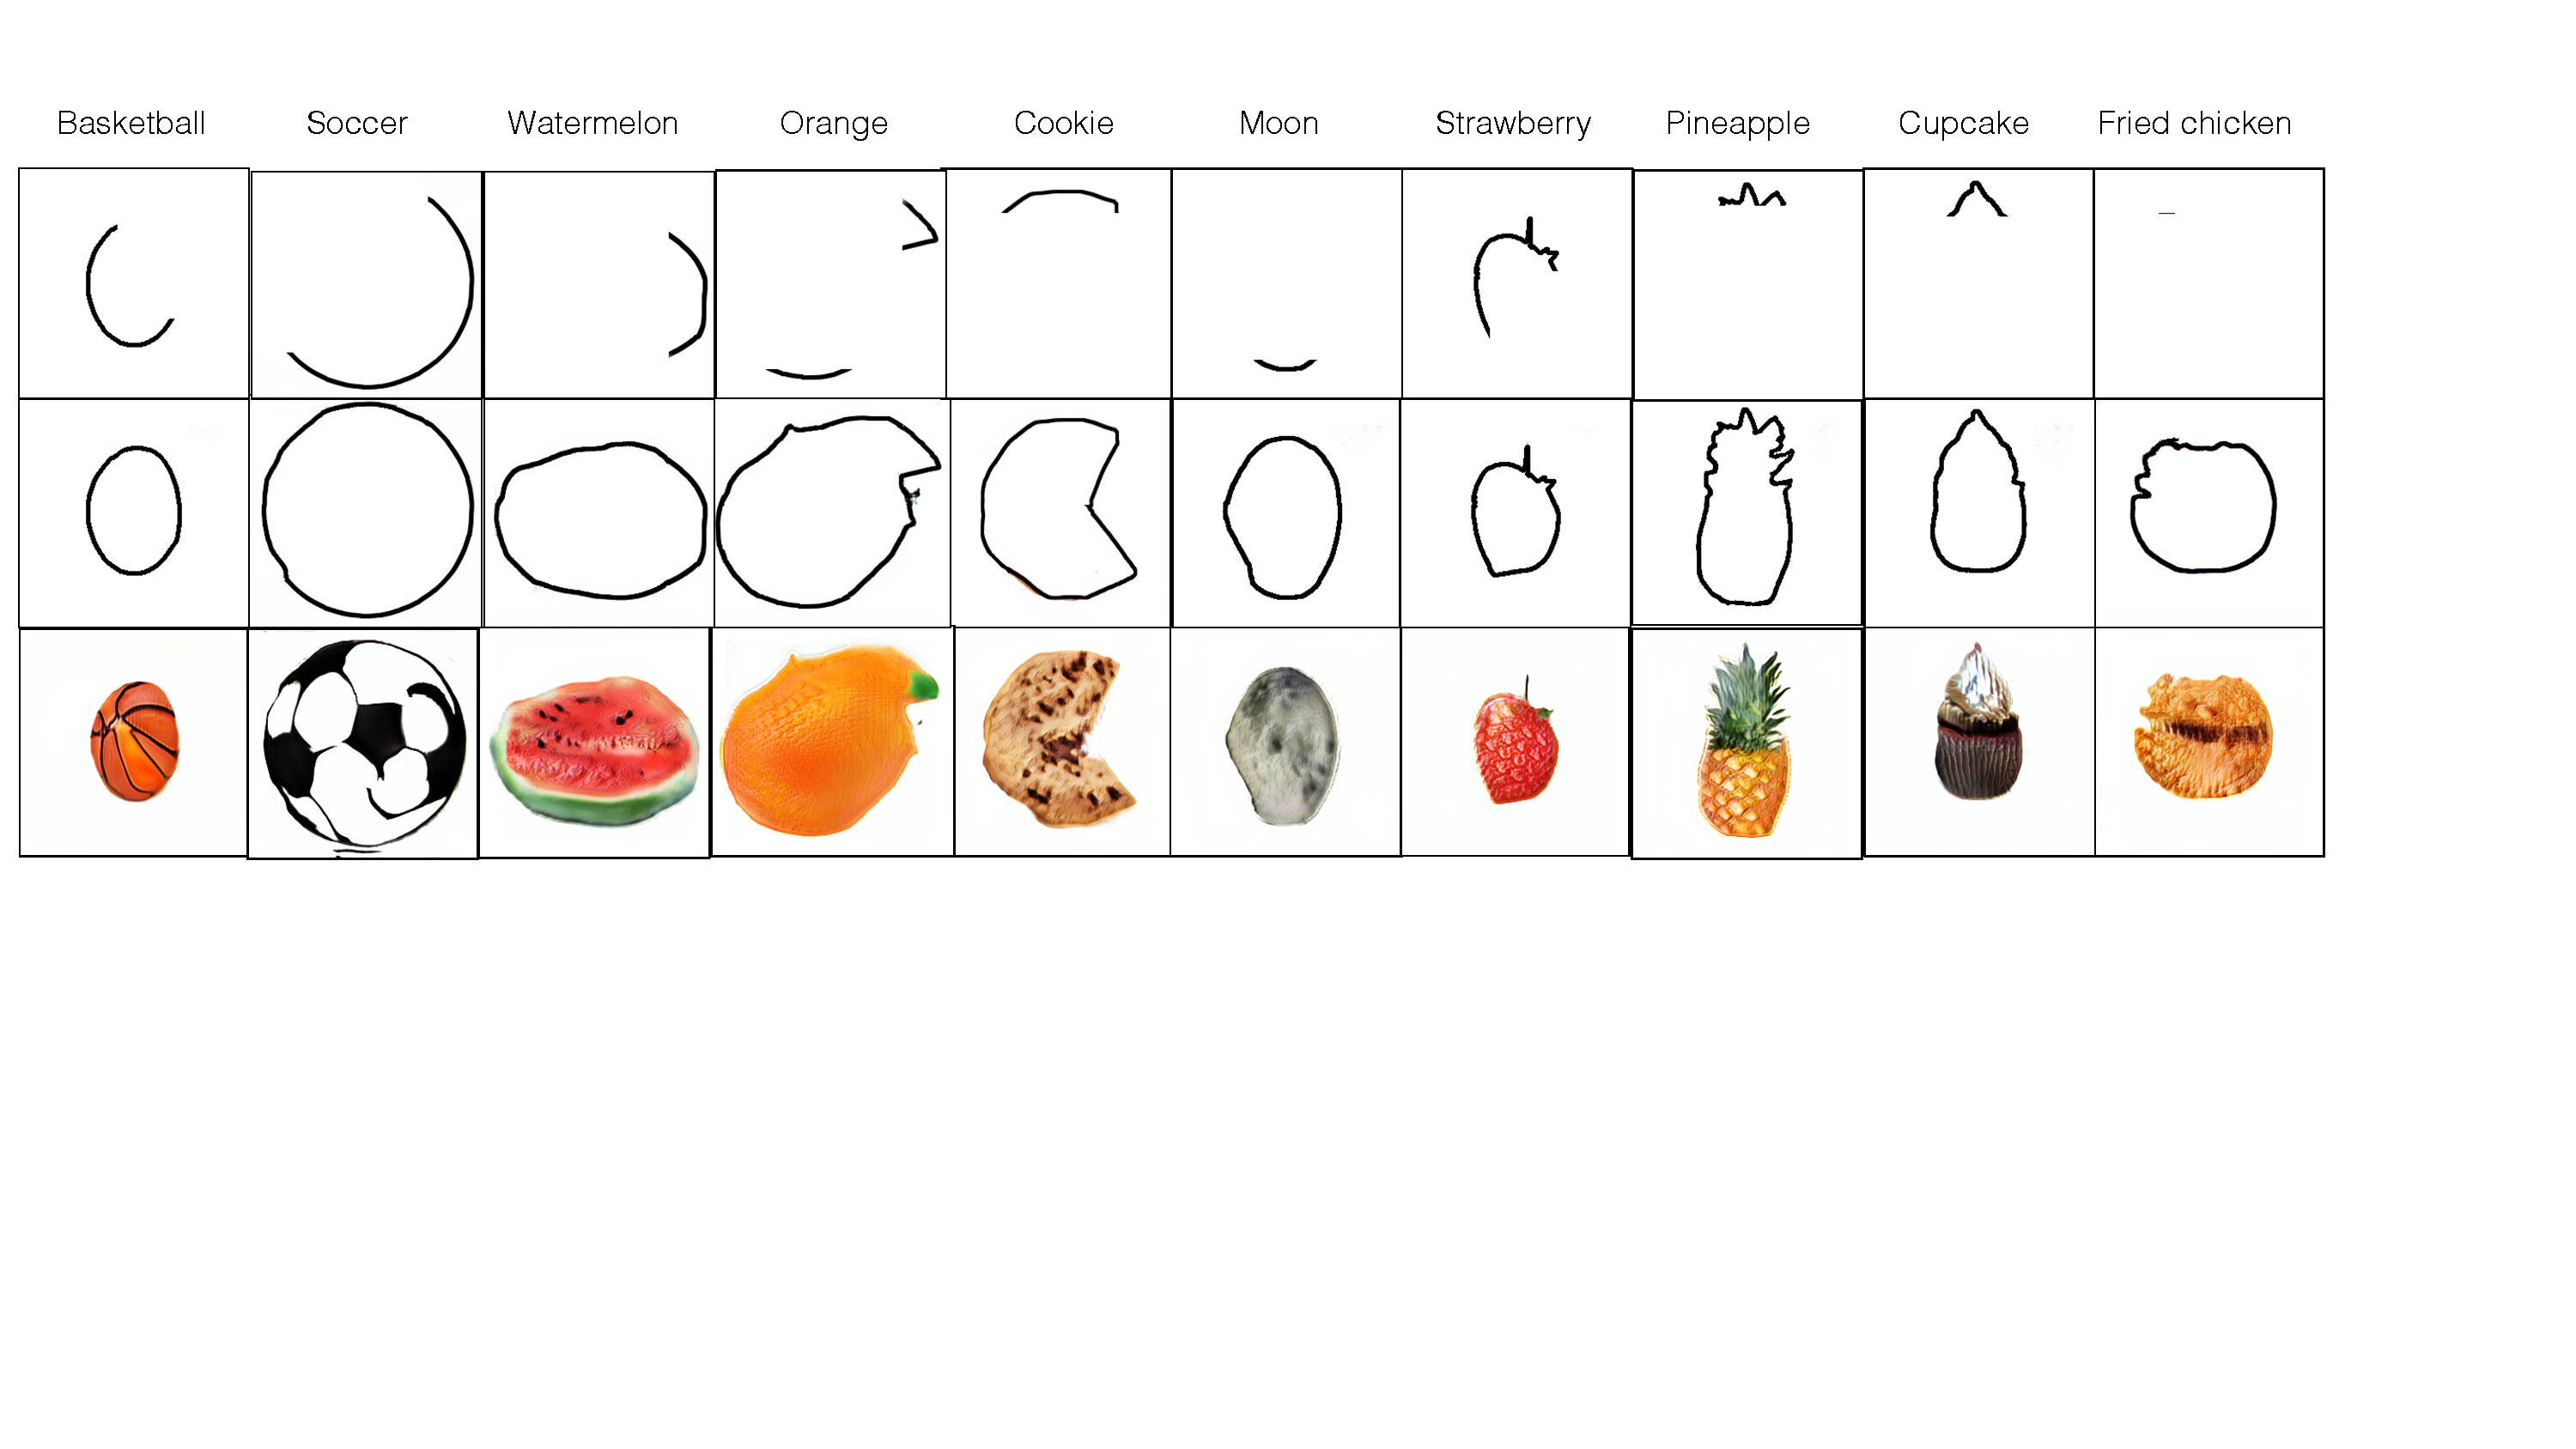
\includegraphics[width=1\linewidth]{paper_images/autocomplete_generate_v1.pdf}
%     \vspace{-15mm}
%     \caption{\textbf{Complete \& Generate results}.
%     A few strokes as shown in the first row is enough to automatically complete the class specific outlines and further generate class specific generations. \es{replace orange and chicken. maybe also moon and cupcake.}}
    
%     % \ow{seems like this is missing 1. two generators, and 2. one generator. instead it seems more like an ablation study on our method, which is not the point. would be more impressive to show it matches 2 generators and 1 generator totally fails.}
    
%     \label{fig:autocomplete_generate}
%     % \vspace{-35mm}
% \end{figure*}


\begin{table}[t]
    \centering
        \begin{tabular}{l c}
        % \hline
        \toprule
        \textbf{Trained task} & \textbf{Avg Acc} \\ \midrule
        % PE $\rightarrow$ Image & 73.12 \% \\
        % PO $\rightarrow$ Image & 88.74 \% \\
        % EC $\rightarrow$ FE $\rightarrow$ Image & 45.96 \% \\
        % OC $\rightarrow$ FO $\rightarrow$ Image \textbf{[Ours]} & \textbf{97.38\%}  \\
        Partial edges $\rightarrow$ Image & 73.12 \% \\
        Partial outline $\rightarrow$ Image & 88.74 \% \\
        Partial edges $\rightarrow$ Full edges $\rightarrow$ Image & 45.96 \% \\
        % \cdashline{1-2}
        Partial outline $\rightarrow$ Full outline $\rightarrow$ Image [Ours] & \textbf{97.38\%}  \\
        \bottomrule %inserts single line
        \end{tabular}
    \caption{\label{table:2step_eval} \textbf{Shape + Appearance Generation Evaluation}. We evaluate the result quality from different task pipelines. Accuracy is computed by a fixed, pretrained classification network, on the resulting images.
    % Evaluates the result quality from different trained task pipelines, including Partial Edges (PE), Partial Outlines (PO), Edge Completion (EC), Full Edges (FE), Outline Completion (OC), and Full Outlines (FO). Accuracy is computed by a fixed, pretrained classification network, on the resulting images.
    }
\end{table}


\begin{figure}[t]%[ht!]
\centering
\begin{tabular}{*{4}{c@{\hspace{3px}}}}
    \frame{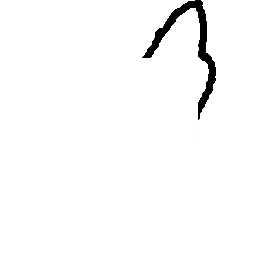
\includegraphics[cfbox=blue 1pt 1pt,width=.22\linewidth]{images/outlines2edges/partial_outline.png}} &
    \frame{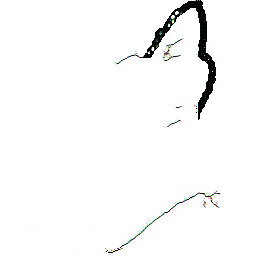
\includegraphics[width=.22\linewidth]{images/outlines2edges/partial_outline_edge_complete.png}} &
    \frame{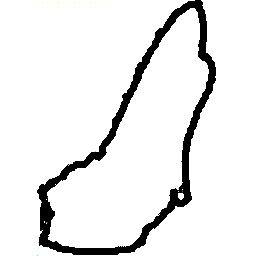
\includegraphics[cfbox=blue 1pt 1pt,width=.22\linewidth]{images/outlines2edges/full_outline.png}} &
    \frame{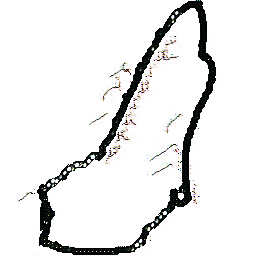
\includegraphics[width=.22\linewidth]{images/outlines2edges/full_outline_edge_complete.png}}
    \\
    
    % \begin{subfigure}[t]{.25\linewidth}\caption{}\label{fig:basketball_partial}\end{subfigure} &
    % \begin{subfigure}[t]{.25\linewidth}\caption{}\label{fig:basketball_full}\end{subfigure} &
    % \begin{subfigure}[t]{.25\linewidth}\caption{}\label{fig:basketball_full}\end{subfigure} &
    % \begin{subfigure}[t]{.25\linewidth}\caption{}\label{fig:soccer_partial}\end{subfigure} \\
\end{tabular} \\
    \caption{\textbf{Partial Outlines $\rightarrow$ Edges} (Trained on edge completion). Blue frames represent inputs to the network. With sparse input, it produces incompatible completions and even if the full outline is provided it fails to produce decent texture strokes.}
    \label{fig:ablation_partial_edge_completion}
    \vspace{-3mm}
\end{figure}


\begin{figure}[t]%[ht!]
\centering
\begin{tabular}{*{6}{c@{\hspace{3px}}}}
    \frame{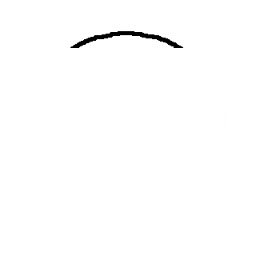
\includegraphics[width=.15\linewidth]{images/ablation_images/basketball_partial_outline.png}} &
    \frame{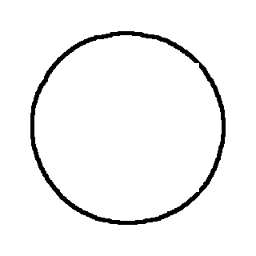
\includegraphics[width=.15\linewidth]{images/ablation_images/basketball_full_outline.png}} &
    \frame{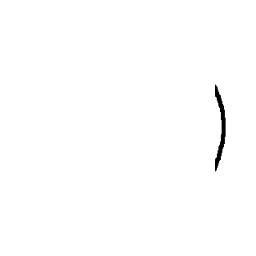
\includegraphics[width=.15\linewidth]{images/ablation_images/soccer_partial_outline.png}} & 
    \frame{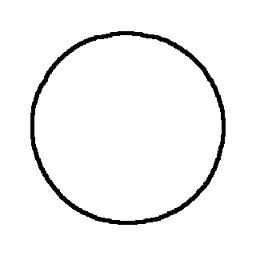
\includegraphics[width=.15\linewidth]{images/ablation_images/soccer_full_outline.png}}&
    \frame{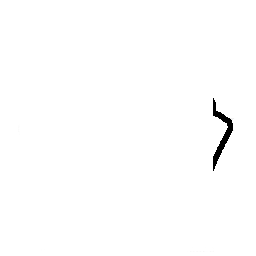
\includegraphics[width=.15\linewidth]{images/ablation_images/cupcake_partial_outline.png}} &
    \frame{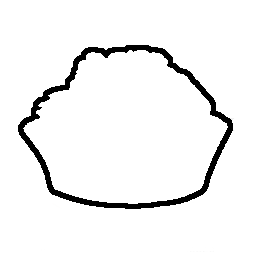
\includegraphics[width=.15\linewidth]{images/ablation_images/cupcake_full_outline.png}}
    \\
    
    \frame{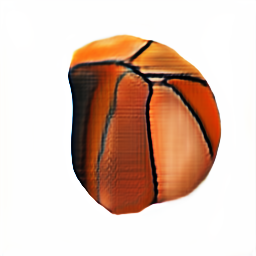
\includegraphics[width=.15\linewidth]{images/ablation_images/basketball_partial_outline_gen.png}} &
    \frame{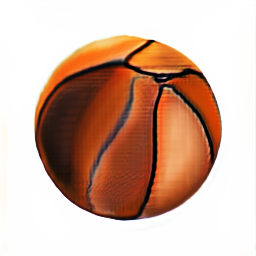
\includegraphics[width=.15\linewidth]{images/ablation_images/basketball_full_outline_gen.png}} &
    \frame{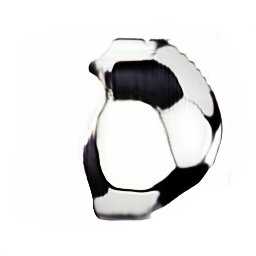
\includegraphics[width=.15\linewidth]{images/ablation_images/soccer_partial_outline_gen.png}} & 
    \frame{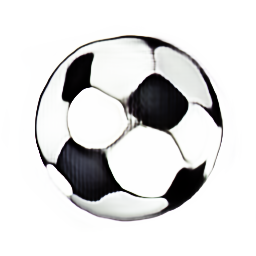
\includegraphics[width=.15\linewidth]{images/ablation_images/soccer_full_outline_gen.png}}&
    \frame{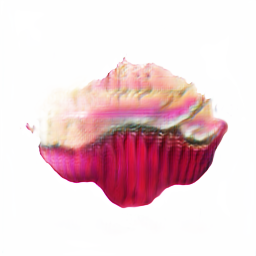
\includegraphics[width=.15\linewidth]{images/ablation_images/cupcake_partial_outline_gen.png}} &
    \frame{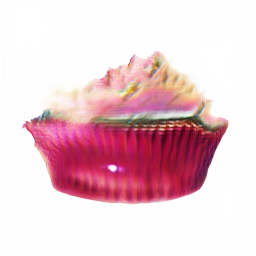
\includegraphics[width=.15\linewidth]{images/ablation_images/cupcake_full_outline_gen.png}}
    \\
    
    % \begin{subfigure}[t]{.15\linewidth}\caption{}\label{fig:basketball_partial}\end{subfigure} &
    % \begin{subfigure}[t]{.15\linewidth}\caption{}\label{fig:basketball_full}\end{subfigure} &
    % \begin{subfigure}[t]{.15\linewidth}\caption{}\label{fig:soccer_partial}\end{subfigure} &
    % \begin{subfigure}[t]{.15\linewidth}\caption{}\label{fig:soccer_full}\end{subfigure} &
    % \begin{subfigure}[t]{.15\linewidth}\caption{}\label{fig:cupcake_partial}\end{subfigure} &
    % \begin{subfigure}[t]{.15\linewidth}\caption{}\label{fig:cupcake_full}\end{subfigure}\\
\end{tabular}
    \caption{\textbf{Direct Partial Outline $\rightarrow$ Image} Illustrating that when the outline is well defined the network can generate nice results but when the outline is sparse the network struggles with the geometry.}
    \label{fig:ablation_partial_full_outline}
    \vspace{-3mm}
\end{figure}



\begin{figure*}[ht!]
  \centering
  \begin{minipage}[t]{0.49\linewidth}  
  \centering
  \resizebox{1.\linewidth}{!} {
  \setlength{\tabcolsep}{6pt}
  \begin{tabular}{l c c c c}
  \toprule
    \multirow{3}{*}{\textbf{Method}} & \multicolumn{2}{c}{ {\bf SkinnyResNet}} & \multicolumn{2}{c}{ {\bf EncDec}} \\ \cmidrule(l){2-3} \cmidrule(l){4-5}
% 	& \textbf{Accuracy} & \textbf{Realism} & \textbf{Accuracy} & \textbf{Realism} \\
	& Class. & AMT Fool. & Class. & AMT Fool. \\
	& Acc [\%] & Rate [\%] & Acc [\%] & Rate [\%] \\ \midrule
% 	\cmidrule(l){1-1} \cmidrule(l){2-3} \cmidrule(l){4-5}
    Ground truth & 100.0 & 50.0 & 100.0 & 50.0 \\ \midrule
    1 gen/class & \textbf{\textit{97.0}} & 17.7$\pm$1.46 & -- & -- \\ \midrule
    Concat (In)	& 62.6 & 15.0$\pm$1.4 & 39.2 & 7.5$\pm$1.06 \\ 
    Concat (All) & 64.5 & 15.3$\pm$1.41 & 51.4 & 5.4$\pm$0.88 \\ \midrule
    Cat(In)+Aux-Class & 65.6 & 14.5$\pm$1.5 & -- & -- \\ 
    Cat(All)+Aux-Class & 67.0 & 19.7$\pm$1.42 & -- & --\\ \midrule
    BlockGate(+bias) & 89.6 & 19.6$\pm$1.34 & -- & --\\ 
    BlockGate & {\bf 99.6} & 17.3$\pm$1.61 & -- & --\\ 
    AdaIn & 94.5 & 14.9$\pm$1.47 & -- & --\\ 
    ChanGate(+bias) & 94.1 & 14.8$\pm$1.43 & -- & --\\ 
    ChanGate & \textbf{\textit{97.0}} & {\bf 23.4$\pm$1.99} & 92.7 & 14.1$\pm$1.48 \\ 
	\hline
	\end{tabular} } 
  \end{minipage}\begin{minipage}[]{0.49\linewidth}
  \centering
  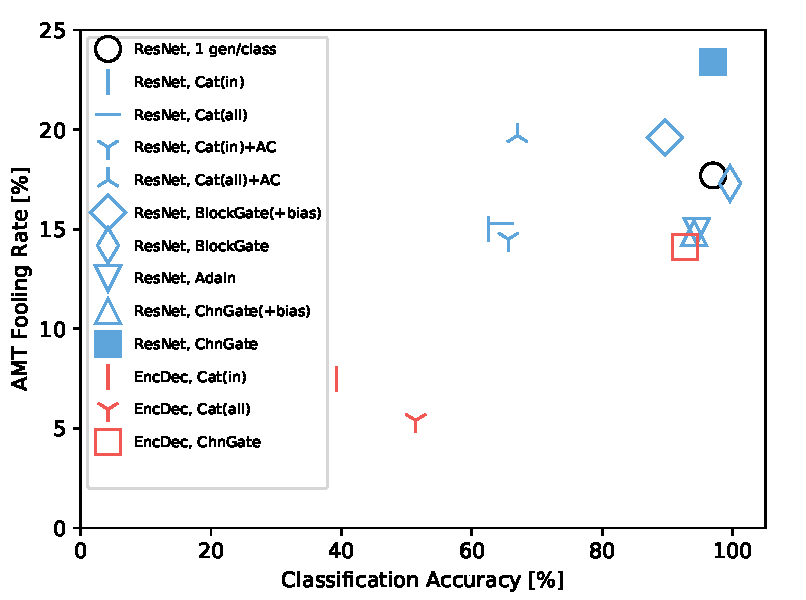
\includegraphics[width=1.\linewidth]{paper_images/gen_real_vs_acc.pdf} 
  \end{minipage}
  \caption{\small {\bf Accuracy vs Realism on Outline$\rightarrow$Image task.} We measure generation accuracy by using a pretrained network to check whether the generated image is of the correct class and realism using the user-judged real vs. fake test from ~\cite{zhang2016colorful,isola2016image2image} conducted on Amazon Mechanical Turk (AMT). Higher is better for both metrics. Our SkinnyResNet architecture outperforms the Encoder-Decoder network, inspired by MUNIT~\cite{huang2018multimodal}. We perform a thorough ablation on our architecture, and find that channel-wise gating achieves high accuracy and higher realism. The right figure shows the correlation between the two tasks.
  \vspace{-4mm}
  }
  \vspace{-3mm}
  \label{fig:acc_vs_real}
\end{figure*}


\begin{figure*}[t]
    \centering
    \includegraphics[width=.9\linewidth]{paper_images/cond_comp2.pdf}
    \caption{{\bf Conditioning injection comparison.} We show results across methods on the outline$\rightarrow$image task using the \textbf{SkinnyResNet} architecture. Naive Concatenation \textbf{Concat} often confuses classes, such as oranges and basketballs, while gating mechanisms such as the \textbf{ChannelGate} method succeed. The gating method also improves results for the \textbf{EncoderDecoder} architecture. \label{fig:alg_comp} }
    \vspace{-4mm}
\end{figure*}


\section{Experiments}
\label{sec:experiments}
%\subsection{Datasets}
To explore the efficacy of our full pipeline, we introduce a new outline dataset, consisting of 200 images (150 train, 50 test) for each of 10 classes -- basketball, chicken, cookie, cupcake, moon, orange, soccer, strawberry,  watermelon and pineapple. The images have all a white background and were collected using search keywords on popular search engines.
% \es{where are images coming from?}
In each image, we obtain rough outlines for the image. We find the largest blob in the image after thresholding it into a black and white image. We fill the interior holes of the largest blob and obtain a smooth outline using the Savitzky–Golay filter~\cite{savitzky1964smoothing}.
% \ow{how?}


\subsection{Shape Completion}

Unlike edge-to-image datasets used in previous~work~\cite{isola2016image2image,zhu2017unpaired,wang2017high}, our outlines are significantly sparser. 
As we show in our experiments, this lets us provide the user with quicker feedback from fewer strokes. 
However, one challenge of using a simplified dataset is that multiple object classes can have similar outlines (e.g., cookie, basketball, orange, moon).
As such, properly integrating conditioning information is essential to be able to generate realistic images across multiple classes.
%This represents better real-life image content that may share geometric properties and forces the sketch-to-image network to effectively integrate class information to be successful in this setting.

As mentioned in~\secref{sec:shape}, we simulate partial strokes in our dataset by removing random square patches and use BicycleGAN~\cite{zhu2017toward} model for training. We show some completion examples in \figref{fig:autocomplete_generate}.
% \pd{Figure here}. 

We evaluate outlines vs edges, and 1-step vs 2-step generation in Table \ref{table:2step_eval}. 
% We use a data generation process on the test set to produce partial edges or outlines on the test set
We use HED edge detector to compute edge maps, and the procedure described in \secref{sec:shape} to compute object outlines for the test set.
We generate multiple occluded edge/outlines to simulate partial user strokes. We then translate, either from the input to image directly, or with a 2-step process. In order to ascertain the quality of generation we use an Inception~\cite{szegedy2016rethinking} network, finetuned on our multi-class dataset. Using off-the-shelf networks to judge the fidelity of results is often used in generation tasks, such as colorization~\cite{zhang2016colorful} and generative modeling~\cite{salimans2016improved}. We report the average classification accuracy over the classes for the generated results by the different techniques.


\paragraph{Why outlines, not edges?} Edges offer the advantage of providing more information about the internal structure of the object. However, as shown in \figref{fig:ablation_partial_edge_completion} \&
\figref{fig:ablation_partialedge_full_outline}, when the network is trained on partial edges (created using the same method as our partial outline dataset) and tested with just a few user strokes, the completion fails miserably. We suspect that this behaviour is due to the increased dependency of the network towards inputs with detailed internal structure. In Table~\ref{table:2step_eval}, for both the 1-step and 2-step pipelines, systems which use partial outlines generate more realistic results than with partial edges.

\paragraph{Why two-stage approach?} As mentioned, partial outline to image generation inherently requires solving two tasks, shape completion (shape generation) and texture filling (appearance generation). As demonstrated in \figref{fig:ablation_partial_full_outline}, in the multi-class dataset when the network is trained on partial outlines to full images, it struggles in generating the right geometry for the missing regions. As shown in Table \ref{table:2step_eval}, given partial inputs, we observe that our 2-step process, using outlines as input, produces generations which are classified more accurately.



\subsection{Appearance Generation}
%\paragraph{Architecture and Gating Comparisons}
We compare our proposed model to the residual \textbf{Encoder-Decoder} model~\cite{huang2018multimodal}.
%In addition, we evaluate and analyze different gating variants and report the most effective one in the context of the outline-to-image generation task.
In addition, we compare our proposed gating strategy and SkinnyResNet architecture to the following methods for  conditional image generation:

\begin{itemize}[noitemsep,leftmargin=12pt]
\item{\bf Per-class}: a single generator for each category; this is the only test setting with \textit{multiple} networks, all others train a single network
\item{\bf Concat (In)}: naive concatenation, input layer only
\item{\bf Concat (All)}: naive concatenation, all layers
\item{\bf Concat (In)+Aux-Class}: we add an auxiliary classifier, both for input-only and all layers settings
\item{\bf BlockGate(+Bias), BlockGate}: block-wise soft-gating, with and without a bias parameter
\item{\bf AdaIn}: Adaptive instance normalization
\item{\bf ChannelGate(+Bias), ChannelGate}: channel-wise soft-gating, with and without a bias parameter
\end{itemize}
AdaIn describes the case where an Instance Normalization~\cite{ulyanovinstance} (IN) operation is applied before scaling and shifting the feature distribution.
We constrain each element of {\boldmath $\alpha$} and {\boldmath $\beta$} in $[-1, 1]$ %(constraining between [0, 1] did not provide the best empirical results).
\vspace{-2mm}
\begin{equation}
X + \mbox{\boldmath $\alpha$} \odot \text{IN} (\mathcal{H}(X)) + \mbox{\boldmath $\beta$}
\end{equation}

% Please see the supplemental material for a more thorough description.
%\pd{Should we put the gating figure? Or refer to the supplementary?}
% \figref{fig:alg_comp} shows the efficacy of Gating on the task outline to image generation. Naive conditioning techniques fail to properly condition the class. Gating allows the condition (class) to be an active part of the generation process which helps the network to easily distinguish different conditions. The Visual Turing Test in terms of Amazon Mechanical Turk's realism scores are shown in \figref{fig:acc_vs_real}.

\vspace{2mm} \noindent \textbf{Evaluation Metrics} We evaluate the results on two axes: adherence to conditioning and realism. We first test the conditioning adherence -- whether the network generates an image of the correct class. Off-the-shelf networks have been previously used to evaluate colorizations~\cite{zhang2016colorful}, street scenes~\cite{isola2016image2image, wang2017high}, and ImageNet generations~\cite{salimans2016improved}. We take a similar approach and fine-tune a pretrained InceptionV3 network~\cite{szegedy2016rethinking} for our 10 classes. The generations are then tested with this network for classification accuracy.
% The class specific generations from the testset were passed through the finetuned network and the classifications were used to judge the class specific purity of the generations.

To judge the generation quality, we perform a ``Visual Turing test" using Amazon Mechanical Turk (AMT). Turkers are shown a real image, followed by a generated image, or vice versa, and asked to identify the fake. An algorithm which generates a realistic image will ``fool" Turkers into choosing the incorrect image. We use the implementation from~\cite{zhang2016colorful}. We show quantitative results in Fig.~\ref{fig:acc_vs_real} and qualitative examples in Fig.~\ref{fig:alg_comp}.

\vspace{2mm} \noindent \textbf{Does naive concatenation effectively inject conditioning?} In Fig.~\ref{fig:alg_comp}, we show a selected example from each of the 10 classes. The per-class baseline trivially adheres to the conditioning, as each class gets to have its own network. However, when a single network is trained to generate all classes, naive concatenation is unable to successfully inject class information, for either network and for either type of concatenation. For the \textbf{EncoderDecoder} network, basketballs, oranges, cupcakes, pineapples, and fried chicken are all confused with each other. For the \textbf{SkinnyResNet} network, oranges are generated instead of basketballs, and pineapples and fried chicken drumsticks are confused. As seen in Fig.~\ref{fig:acc_vs_real}, classification accuracy is slightly higher when concatenating all layers ($64.5\%$) versus only the input layer ($62.6\%$), but is low for both.
% As evident from \figref{fig:alg_comp} for some classes naive concatenation helps in generating appealing images but for some classes it either fails to generate images from the right class or generates unrealistic images from that class.
% No, point to Figure 9 (qualitative grid) \& Figure 10 (the plot)

% \paragraph{Does gating produce accurate and realistic conditional generations?} The gating mechanisms succeeds in generating realistic images from each class while also preserving the class conditioning appropriately. As evident from the comparisons of generations in \figref{fig:alg_comp} and the metrics reported in \figref{fig:conditioning_amt} the channel wise multiplication produces the most visually appealing results amongst the various gating mechanisms.
% Yes, point to Figure 9 results. Also analyze which variation is the best

\vspace{2mm} \noindent \textbf{Does gating effectively inject conditioning?} Using the proposed soft-gating, on the other hand, leads to successful generations. We test variants of soft-gating on the \textbf{SkinnyResNet}, and accuracy is dramatically improved, between $89.6\%$ to $99.6\%$, comparable to using a single generator per class ($97.0\%$).
% \pd{Two variants of gating provide accuracy better than per-class generator.}
Among the gating mechanisms, we find that channel-wise multiplication
% (on both generator and discriminator)
generates the most realistic images, achieving an AMT fooling rate of $23.4\%$. Interestingly, the fooling rate is higher than the per-class generator of $17.7\%$. Qualitatively, we notice that per-class generators sometimes exhibits artifacts in the background, as seen in the generation of ``moon". We hypothesize with the correct conditioning mechanism, the single generator across multiple classes has the benefit of seeing more training data and finding common elements across classes, such as clean, white backgrounds.
% \pd{it can be confusing also. is it a good justification?}
% The classification accuracy of an Inception network finetuned on our dataset demonstrates the purity of the generations corresponding to the correct class using the gating mechanism. 

% As seen in \figref{fig:alg_comp}, all of the various gating mechanisms and the baselines are able to generate images of high quality and realism from some classes but most of the baselines fail in some classes, often mixing visual features from wrong classes. 


\vspace{2mm} \noindent \textbf{Is gating effective across architectures?} 
% We evaluate the following architectures on the outlines-to-images task. 
% We first evaluate our \todo{SkinnyResNet} with a more traditional encoder-decoder architecture. 
% We use the architecture proposed in MUNIT~\cite{huang2018multimodal} which consists of an encoder followed by a set of residual blocks with a decoder at the end.
As seen in Fig.~\ref{fig:acc_vs_real}, using channelwise gating instead of naive concatenation improves performance both accuracy and realism \textit{across} architectures. For example, for the \textbf{EncoderDecoder} architecture, gating enables successful generation of the pineapple.
% In this case, we apply the gating to this architecture only on the bottleneck residual blocks.
% As evident from \figref{fig:alg_comp} although the network learns to disentangle the various classes, the generation quality reduces from the skinny resnet architecture where all the layers are gated.
Both quantitatively and qualitatively, results are better for our proposed \textbf{SkinnyResNet} architecture.

% Yes, works for both skinny resnet \& enc-dec.

\vspace{2mm} \noindent \textbf{Do the generations generalize to unusual outlines?} The training images consist of the outlines corresponding to the geometry of each class. However, an interesting test scenario is whether the technique generalizes to unseen shape and class combinations. In \figref{fig:teaser}, we show that an input circle not only produces circular objects, such as a basketball, watermelon, and cookie, but also noncircular objects such as strawberry, pineapple, and cupcake. Note that both the pineapple crown and bottom are generated, even without any structural indication of these parts in the outline.


%To additional validate our approach on existing edges2shoes and edges2handbags datasets~\cite{isola2016image2image}.
%Previous work~\cite{isola2016image2image,sangkloy2017scribbler,zhu2017unpaired,wang2017high} trained edge-to-image translation networks, have been applied to the sketch-to-image problem domain.
%\ow{have to add why we dont use datasets from them}
%, sometimes gaining unexpected popularity\footnote{Edges to cats demo: https://affinelayer.com/pixsrv/}. 
%Therefore, we introduce our own dataset, 
%and obtain rough outlines for each image. %using Adobe Photoshop
% Unlike previous work on scribble-to-image translation 

% , as the internal features must be learned by the network, and the same outline can generate substantially different images conditioned on different classes.
% , as seen in Fig.~\ref{fig:teaser}.
%The task involves multiple different objects of high realism when the input is very similar for the various classes several of them being exactly same(in the case of circular objects where the input scribble is an identical scribble for all circular classes). 



%Practically speaking, using the data generation process in which random chunks of the edgemap are occluded, it is hard for the network to discern which parts are missing by design and which parts are missing by random chance and becomes a much harder problem for the shape generation network. 
%When the shape generation network is trained on partial outlines, occlusion indicates the regions where the network has to accurately fill the endpoints with a curve that represents the geometry of the boundary for that particular class. Since variations in each class geometry is limited, this task is relatively easier than filling the edgemap. 
%While having a system that can recommend abstract shape completion from arbitrary internal edges would be useful, we believe it is of extreme importance, we believe that it requires specific architecture and loss design, along with careful data augmentaion, and leave it as a future problem to work on. Outline to real generations is the first step in that direction.


%particular class while if the generation network is given the full completed outline it generates quite plausible results for that particular category. 
%In fact, training produces even better results than just training on outline to images in a similar vein why denoising autoencoders \cite{vincent2010stacked} work better than simple autoencoders.
% since the automated procedure creates a \pd{regularization effect and the network has to work harder in order to generate realistic texture from the sparse user inputs. not sure about this.}

%As shown in \figref{fig:ablation_partial_full_outline} when the network is trained with partial outlines and partial edges and tested with just a few user strokes both fail to generate realistic generations. As shown in the second row, when a pretrained network trained on edges2shoes is tested with just the boundary it generates a silver shoe although it misses out on generating realistic texture cues since the training data consisted of texture cues in the map and the translation network could rely on the texture cues provided in the input edge map and without its presence its unable to produce realistic generation. The network trained on outlines to real images is capable of generating realistic shoe images from an automatically completed outline from the sparse user cues thus showing the efficacy of the 2 step process. 

%\es{why is this interesting? The only interesting case is when the input is sparse outline strokes as we expect to have from a novice user. Partial edge maps as an input are less interesting, and don't deserve a special figure and half a page of text, I think.}

%\es{This section needs a major rewrite. It seems like it is not only about outlines vs. edges but about why our two stage network (partial outlines-full outlines-image) is better than a one stage (partial outlines->image), as well as the analogues with edge maps - (partial edges-full edges->image) and (full edges->image). We don't have to describe the failures of other variants, just point to the user study table and ref to the figure for a visual comparison.}



% \subsection{Two-Stage Shape and Appearance Generation Evaluation}

%\paragraph{Why direct appearance synthesis from partial outlines $\rightarrow$ images not efficient?}


%For the shape completion network, we use the BicycleGAN model~\cite{zhu2017toward}, and for the image generation network, we use a gated SkinnyResNet model so take full advantage of the class conditioning. 
%We first describe our dataset (new) which contains pairs of sparse scribbles and images.
%As seen in \figref{fig:autocomplete_generate} with just a few strokes the user is able to generate full images belonging to their desired class.

% \subsection{Multimodal Generation}
% \label{sec:multimodal}

% %We also tested the efficacy of gating on the task of generating diverse results in the Image-to-Image setting, an important open problem~\cite{isola2016image2image}. 
% %We experimented with the InfoGAN~\cite{chen2016infogan} setting where a Q network tries to reconstruct back a randomly sampled conditioning vector used for generating a sample by the generator. 
% %With a simple gating network, diverse outputs could be generated thus showing the efficacy of gating in handling multiple modes of the data distribution (see Sec.~\ref{sec:multimodal}). Na\"{\i}ve concatenation techniques in this setting had previously proved to be not effective as demonstrated in \cite{zhu2017toward} and complicated techniques such as BicycleGAN \cite{zhu2017toward}, MAD-GAN \cite{ghosh2017multi} had to be introduced.
% %\ow{move this above paragraph into the actual experiments. no need to warn people about experiments that are going to come when its the immediate next section}

% Inter-class variation, also called diversity, is a significant challenge in GAN image generation applications. 
% In the pix2pix setting, as shown by previous works \cite{ghosh2017multi} and \cite{zhu2017toward} even the InfoGAN (cLR in \cite{zhu2017toward}) setup was not able to produce meaningful variations (irrespective of the variations in the conditioning), and additional generators or cyclical losses were required to produce meaningful variations in the generated images. 
% With our gating mechanism, we show that we can create meaningful variations, using just the InfoGAN objective.
% This can be seen in the results \figref{fig:infogan_gate} and from the LPIPS metric \cite{zhang2018unreasonable} in  Table. \ref{table:infogan_lpips} which measures the diversity among the generations in the feature space of a standard Imagenet classifier.
% % Since InfoGAN maximizes mutual information, we argue that gating provides a mechanism to effectively optimize it by making the conditioning an active part of the generation process (refer Sec.~\ref{sec:infoGAN}).

% \begin{figure}[h]
%     \centering
%     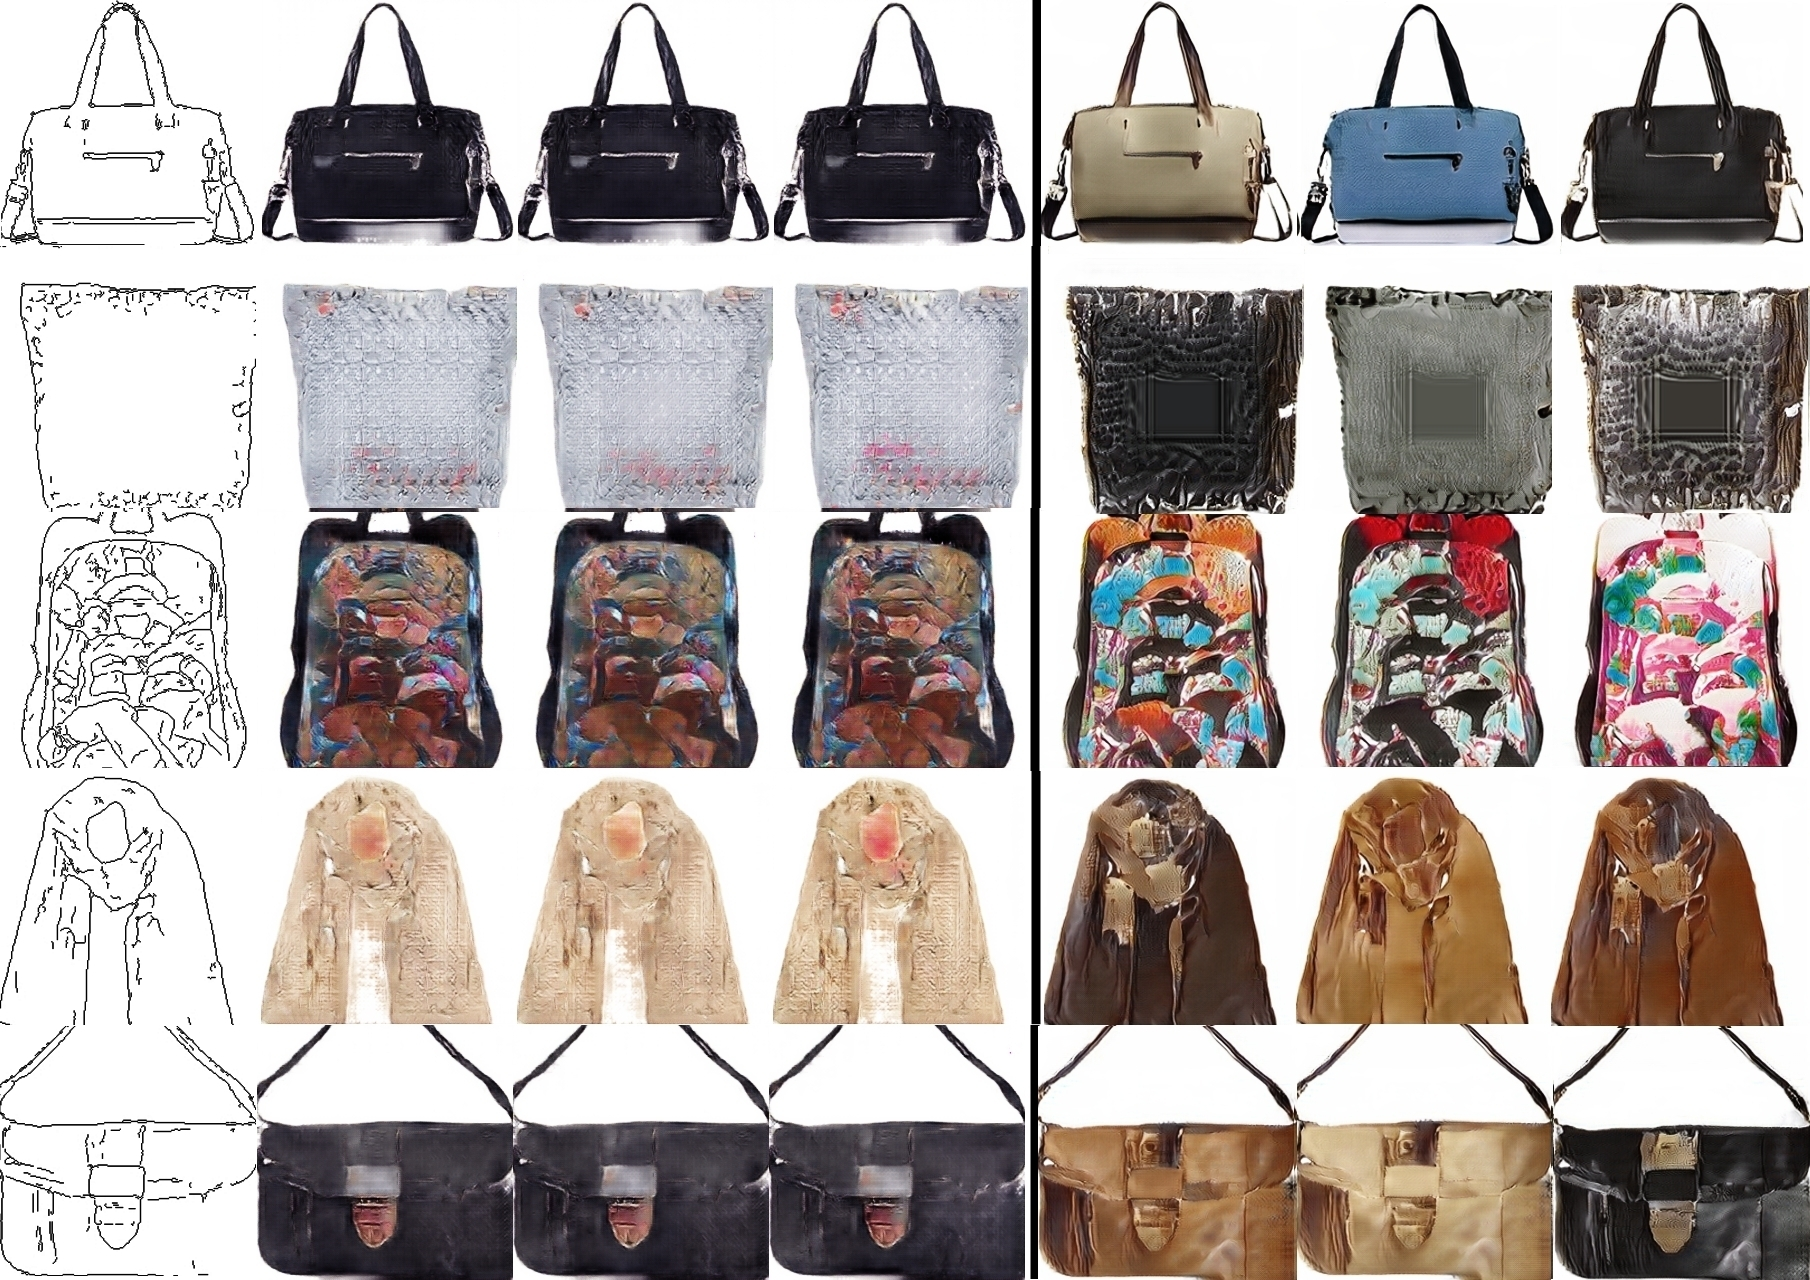
\includegraphics[width=\linewidth]{infogan.jpg}
%     \caption{{\bf Edges$\rightarrow$Handbags qualitative examples.} Naive Conditioning of InfoGAN fails (left) while gating (right) succeeds in producing diverse generations.
%     \vspace{-5mm}
%     }\label{fig:infogan_gate}
%     \vspace{-2mm}
% \end{figure}
% \begin{table}[h]
%     \centering
%         \begin{tabular}{l c}
%         % \hline
%         \toprule
%         \textbf{Model} & \textbf{LPIPS Distance} \\ \midrule
%         Random Real Images & $0.3665 \pm 0.0053$ \\ \midrule
%         BicycleGAN~\cite{zhu2017toward} & $0.1374 \pm 0.0005$  \\ \midrule
%         Concat(In) &  $0.0432 \pm 0.0002$ \\
%         Concat(All) & $0.0159 \pm 0.0004$ \\ \cdashline{1-2}
%         ChannelGate [Ours] & $0.0964 \pm 0.0003$  \\
%         \bottomrule %inserts single line
%         \end{tabular}
%     \caption{\label{table:infogan_lpips} {\bf Edges$\rightarrow$Handbags Diversity.} LPIPSv0.1~\cite{zhang2018unreasonable} distance between randomly generated handbags, given the same edge map, as proposed in~\cite{zhu2016generative}. Given the same architecture, gating achieves higher diversity than concatenation.}
% \end{table}


% \subsection{Autocomplete Data Generation:}

% \begin{figure}[h!]%[ht!]
% \centering
% \begin{tabular}{*{4}{c@{\hspace{3px}}}}
%     \frame{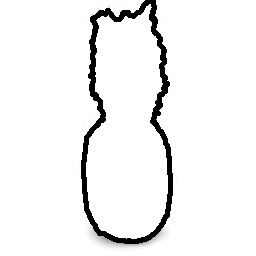
\includegraphics[width=.22\linewidth]{images/autocomplete_data_generation/original.png}} &
%     \frame{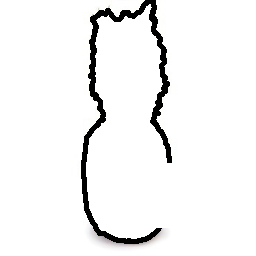
\includegraphics[width=.22\linewidth]{images/autocomplete_data_generation/64.png}} &
%     \frame{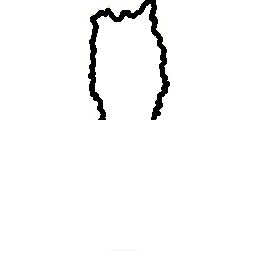
\includegraphics[width=.22\linewidth]{images/autocomplete_data_generation/128.png}} &
%     \frame{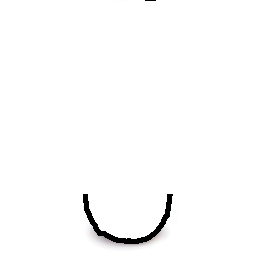
\includegraphics[width=.22\linewidth]{images/autocomplete_data_generation/192.png}}\\
%     \vspace{-1mm}
%     \begin{subfigure}[t]{.22\linewidth}\caption{Outline}\end{subfigure} &
%     \begin{subfigure}[t]{.22\linewidth}\caption{64x64}\end{subfigure} &
%     \begin{subfigure}[t]{.22\linewidth}\caption{128x128}\end{subfigure} &
%     \begin{subfigure}[t]{.22\linewidth}\caption{192x192}\end{subfigure} \\
% \end{tabular} \\
%     \caption{\textbf{Autocomplete Training Data Creation:} 3 sizes (64x64,128x128,192x192) of white colored occluders were used for simulating partial edges }
%     \label{fig:autocomplete_data_generation}
%     \vspace{-3mm}
% \end{figure}





% \section{Experiments Old}

% % \begin{figure}[t]
% %     \centering
% %     \vspace{-20mm}
% %     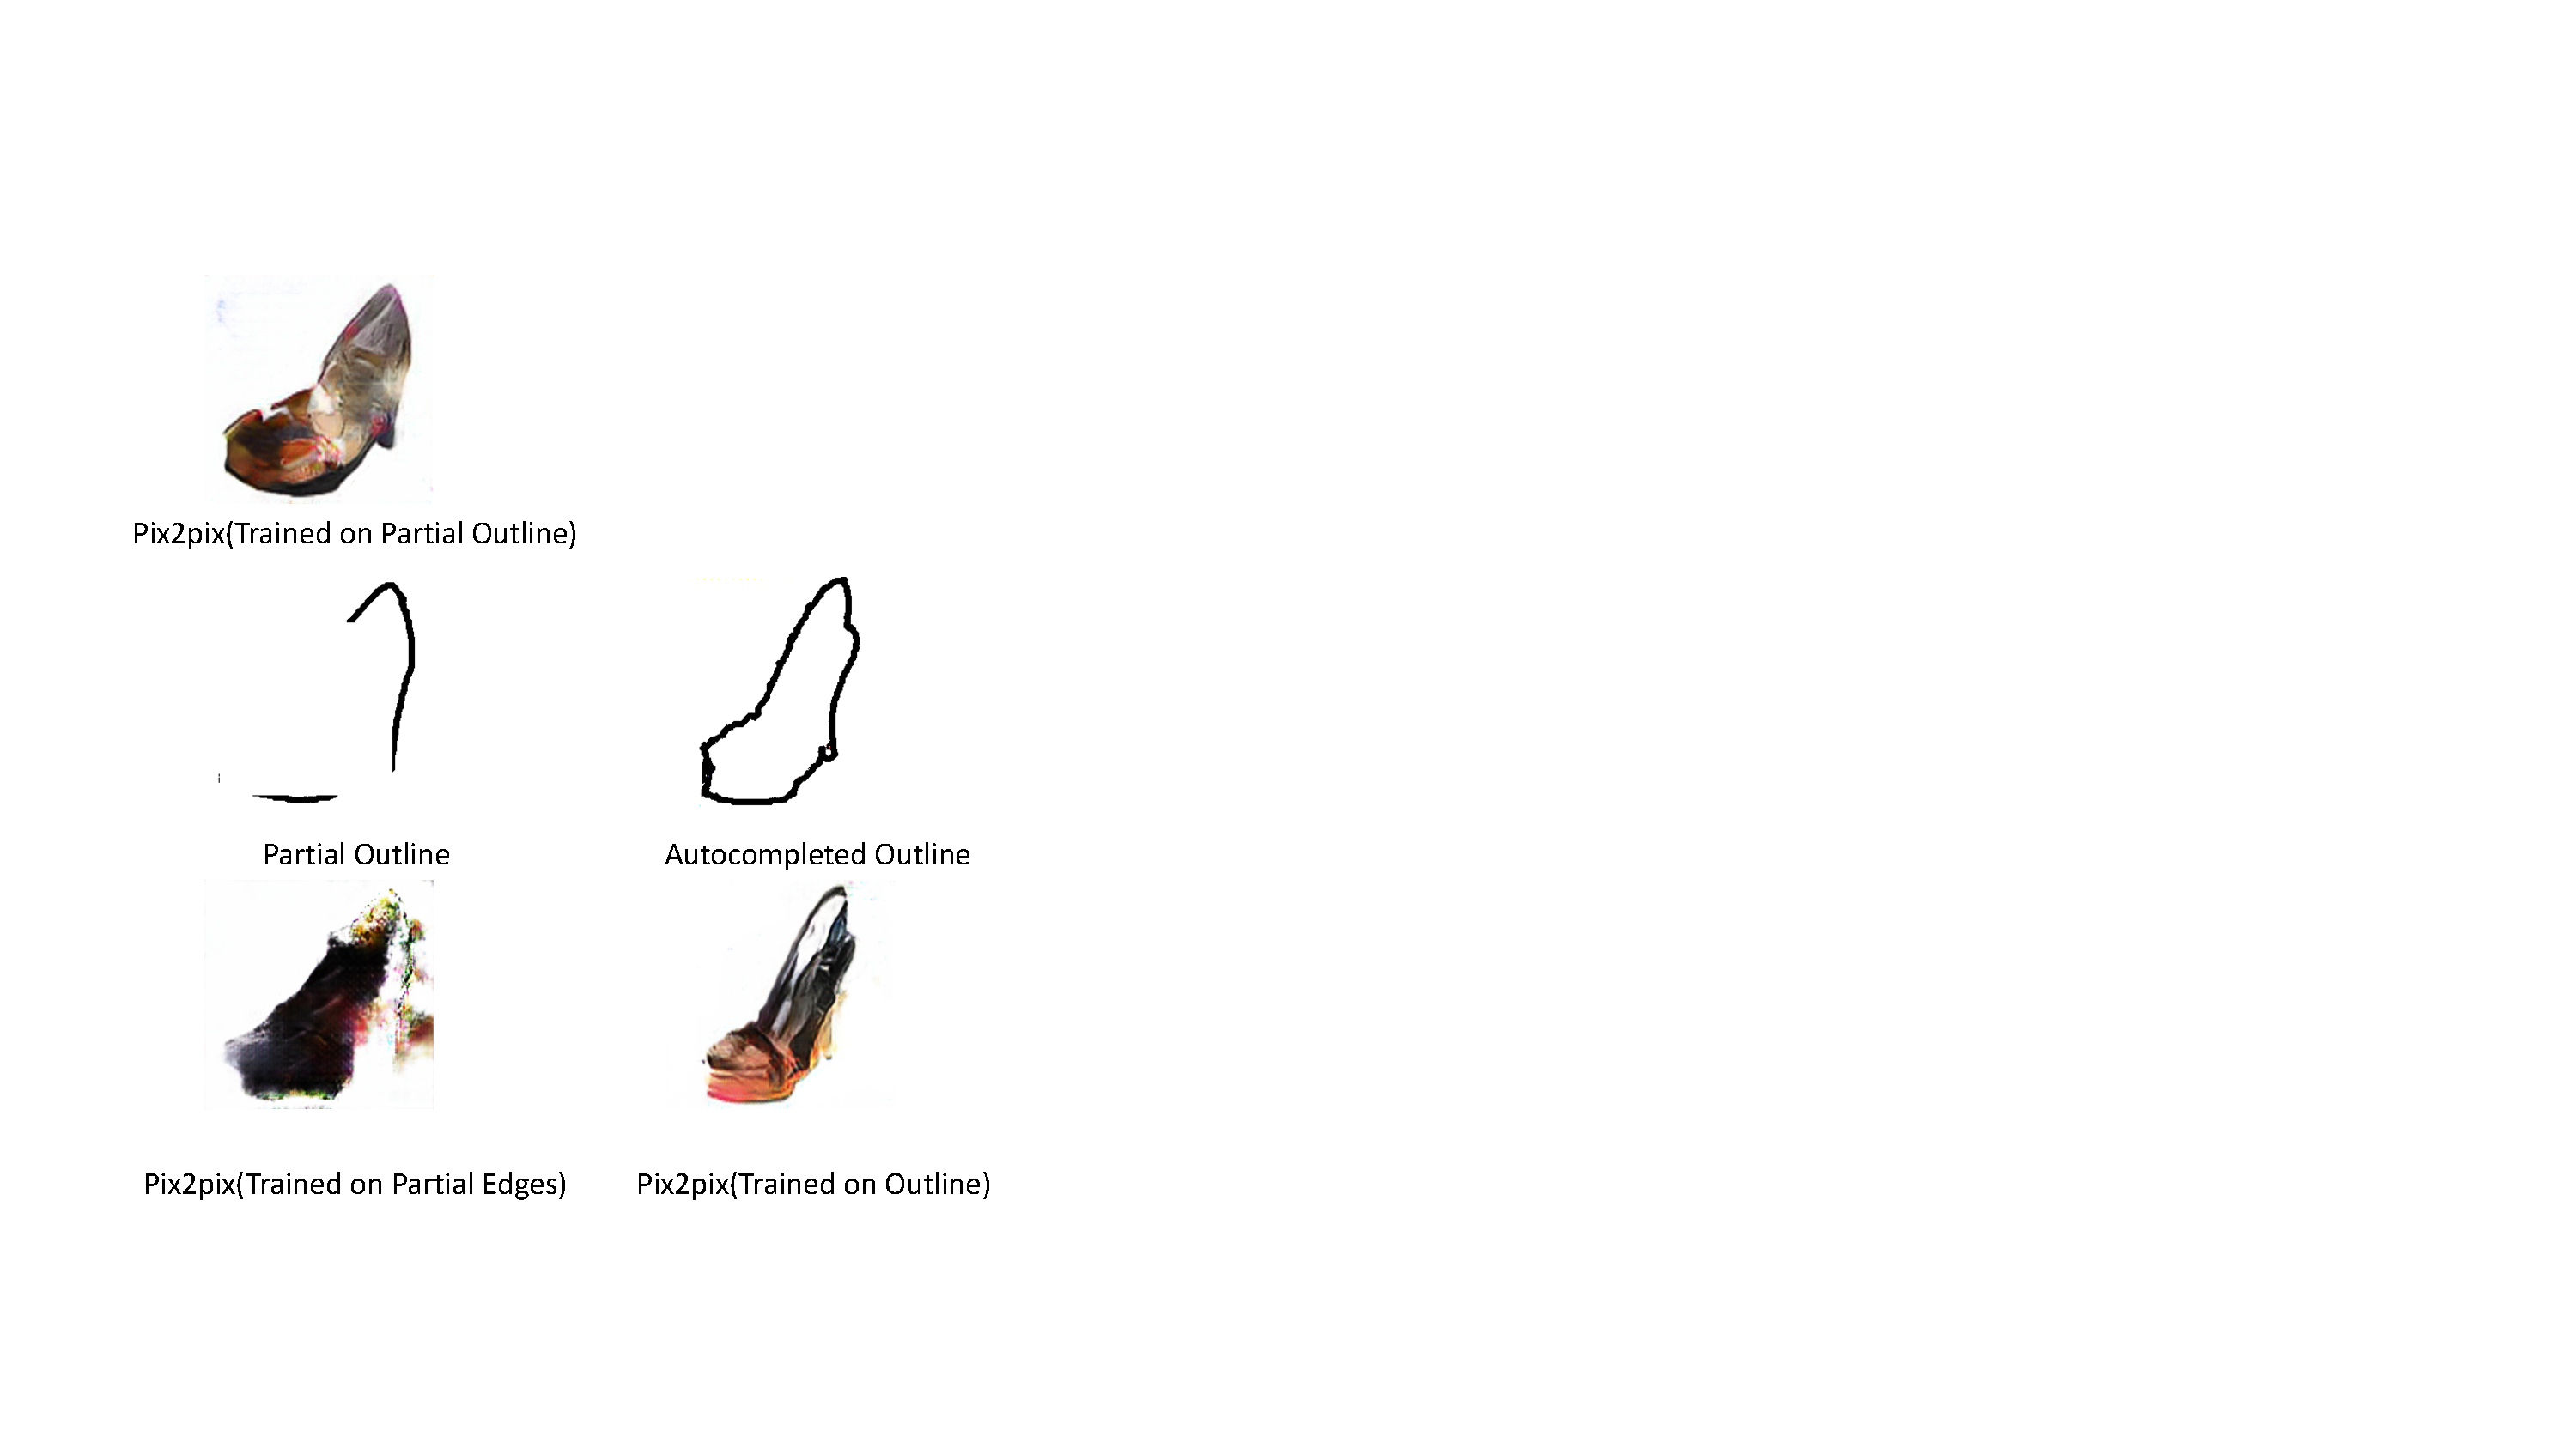
\includegraphics[width=2.5\linewidth]{paper_images/ablation_edges_outlines_shoes.pdf}
% %     \caption{\textbf{Shoe generation results}. Generating realistic images trained with partial sketches or partial outlines fails when large chunks of the input sketch/outline is missing while images trained via a 2 step process of first generating the outline and then generating the real image from the completed outline generates better results}
% %     \vspace{-15mm}\label{fig:infogan_gate}
% %     \vspace{-2mm}
% % \end{figure}

% % \begin{figure}[t]
% %     \centering
    
% %     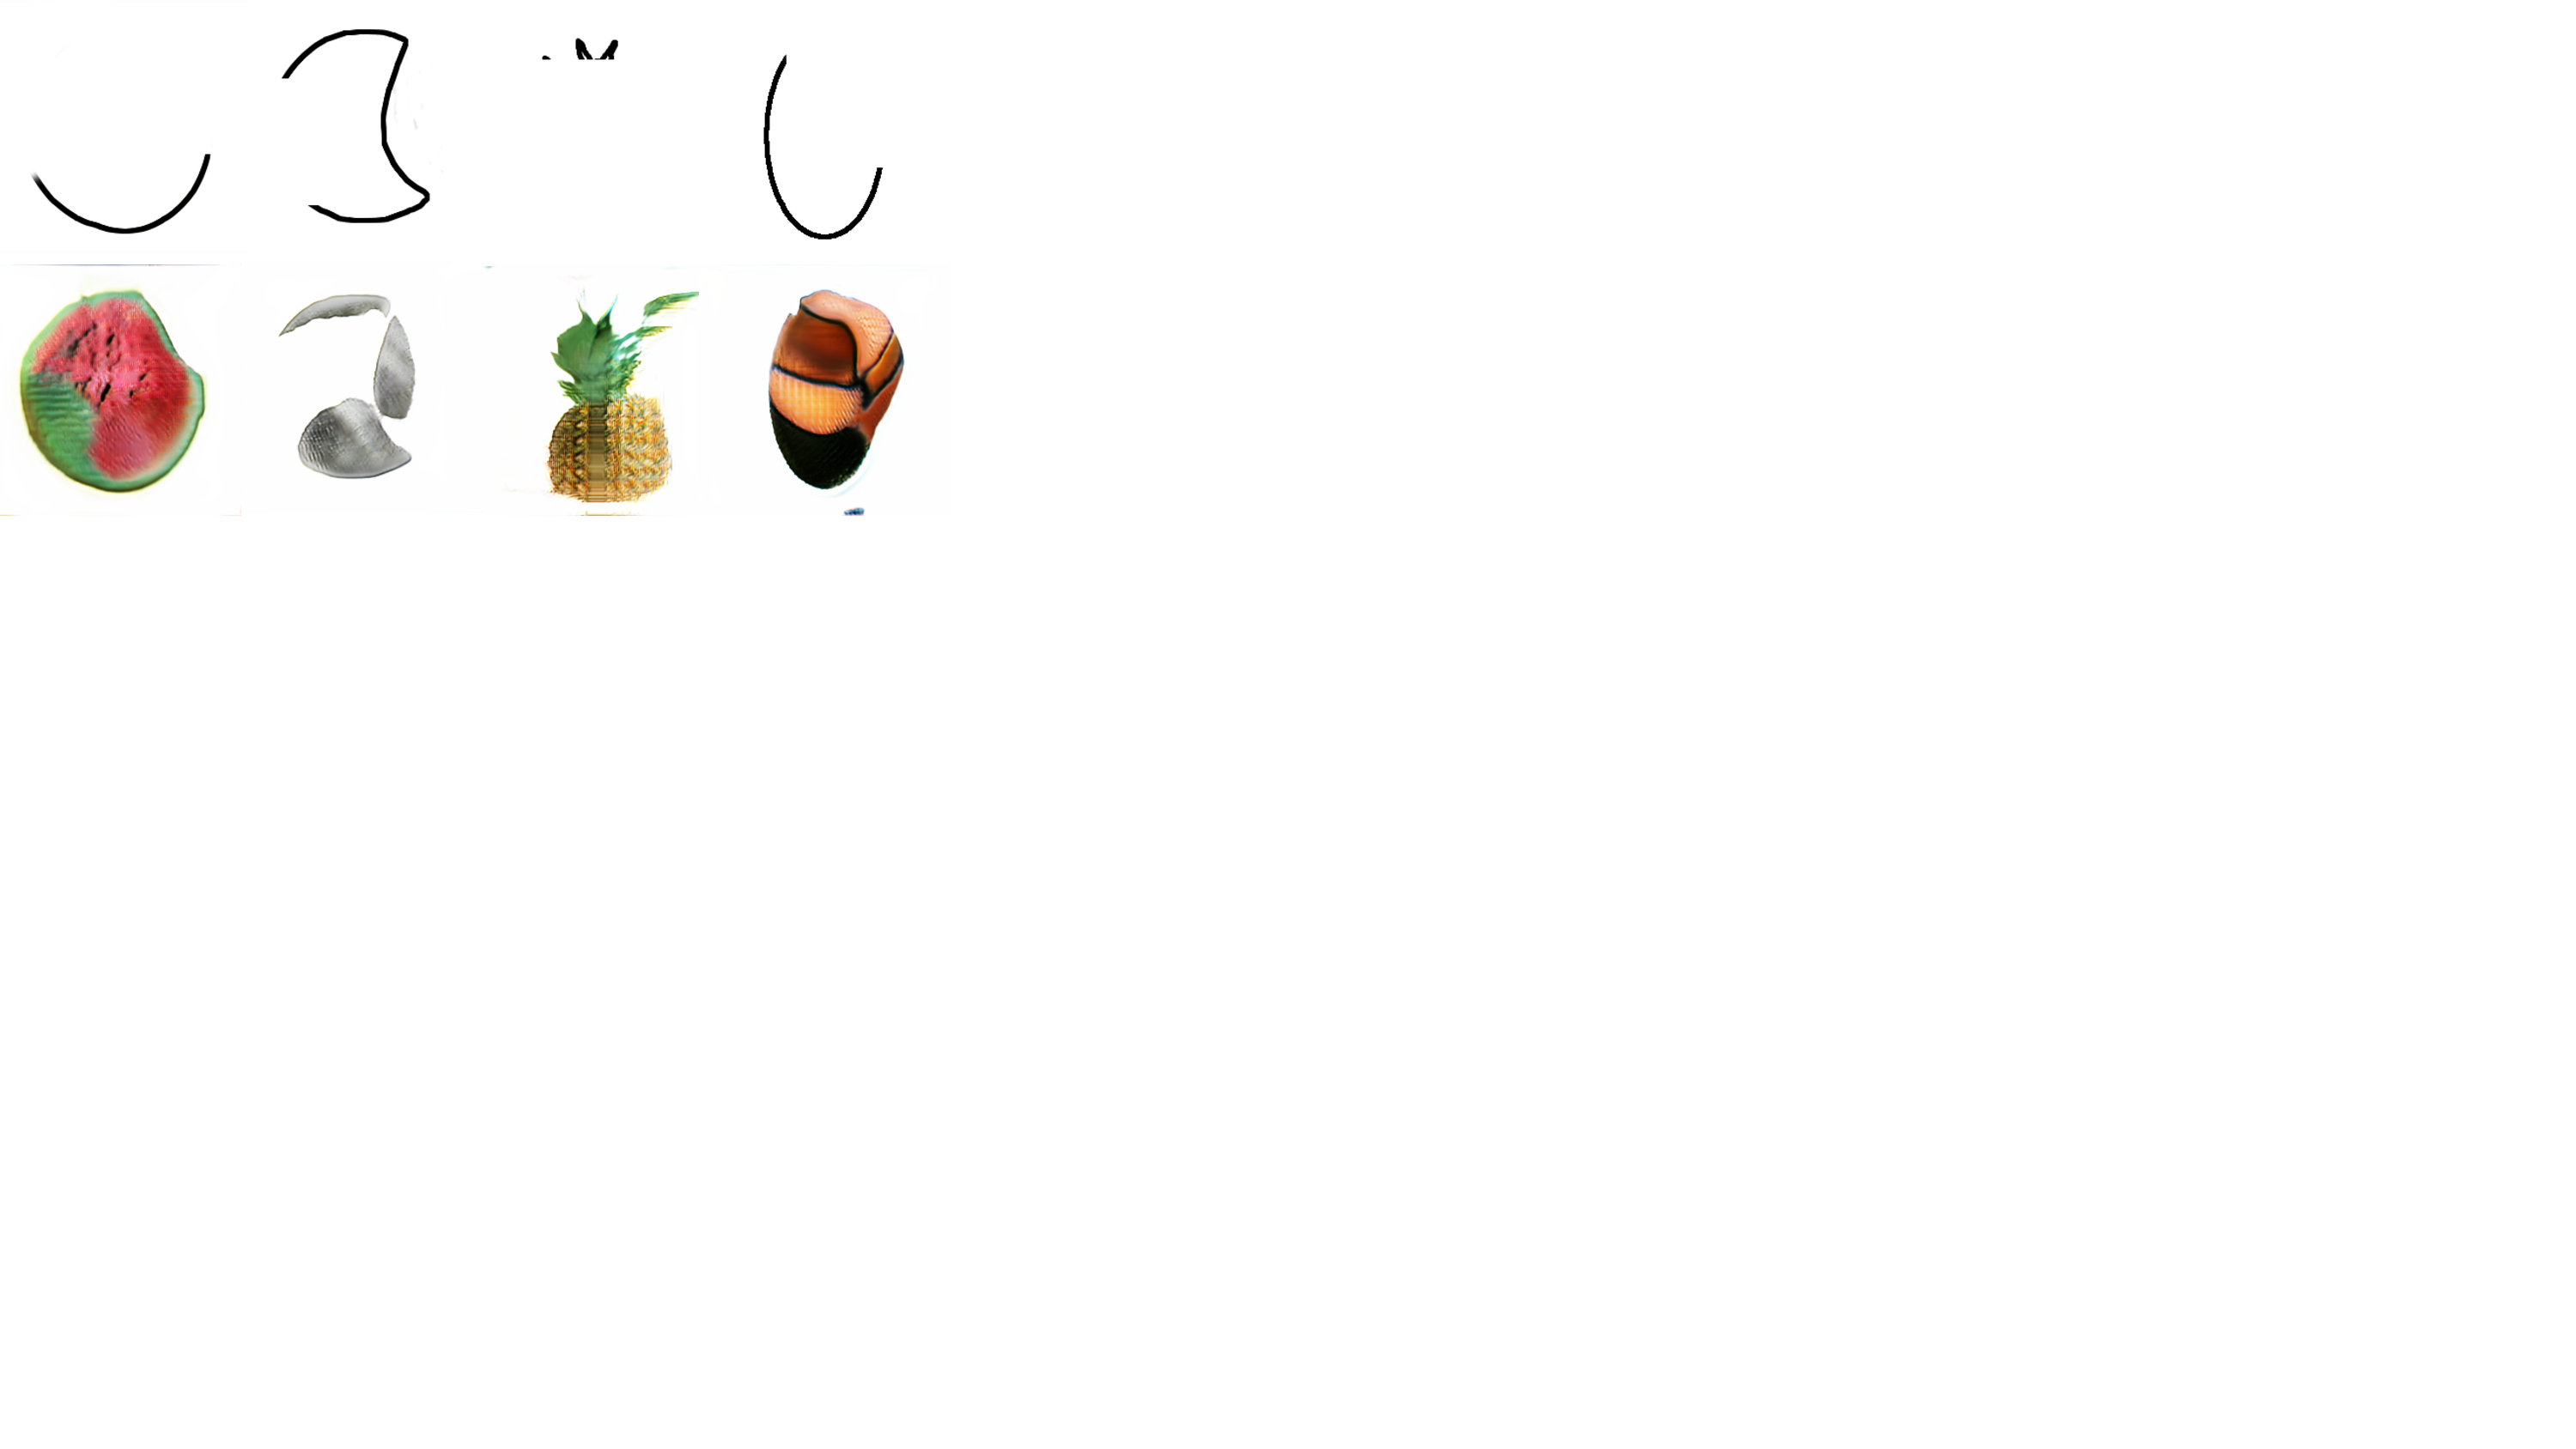
\includegraphics[width=2.5\linewidth]{paper_images/outline_direct_failure_multi_class.pdf}
% %     \vspace{-60mm}
% %     \caption{\textbf{Outline $\rightarrow$ Image generation results trained with partial outlines}. When directly trained from partial outlines to RGB images when large parts of the image are missing, the generator falters in geometry or texture.}
% %     \vspace{-15mm}\label{fig:infogan_gate}
% %     \vspace{-2mm}
% % \end{figure}

% % \begin{figure}[t]
% %     \centering
% %     \vspace{-20mm}
% %     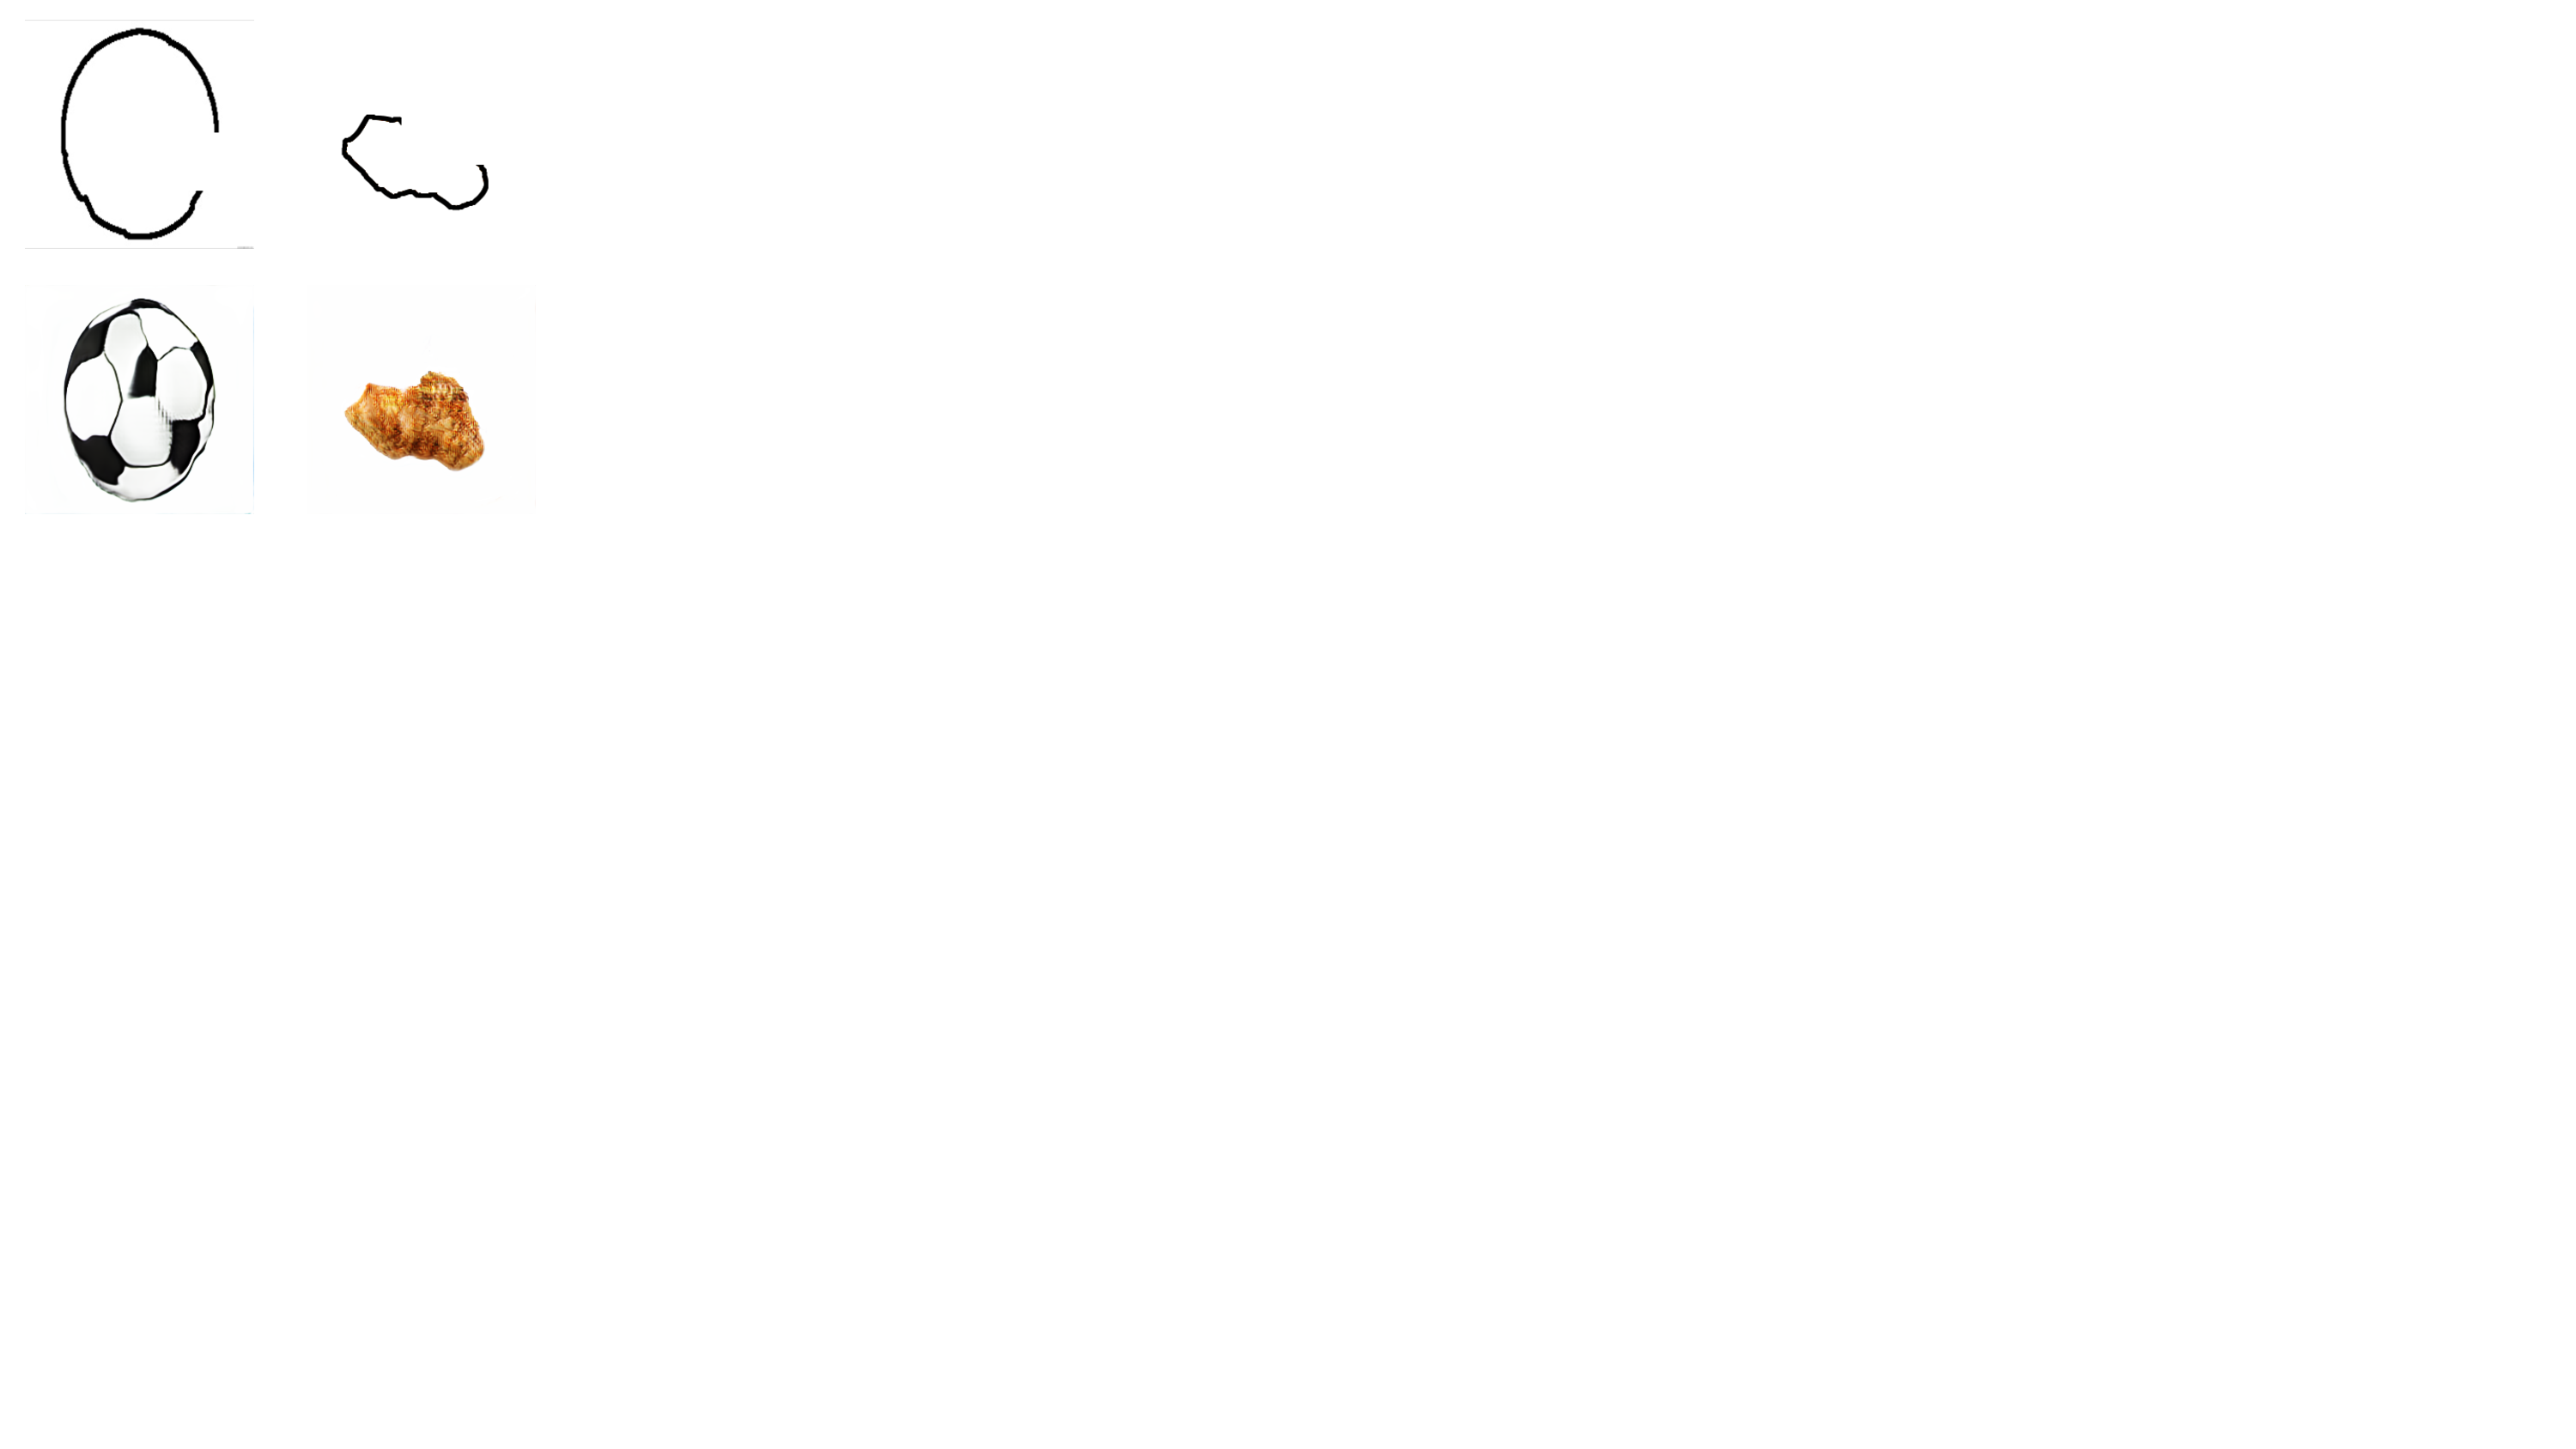
\includegraphics[width=3\linewidth]{paper_images/success_multiclass.pdf}
% %     \vspace{-35mm}
% %     \caption{\textbf{Success Of Partial Outlines $\rightarrow$ Image:} When the input sketch is almost complete, it generates decent results. }
% %     \label{fig:infogan_gate}
% %     \vspace{-2mm}
% % \end{figure}
% % \begin{figure*}[h]
% %     \centering
% %     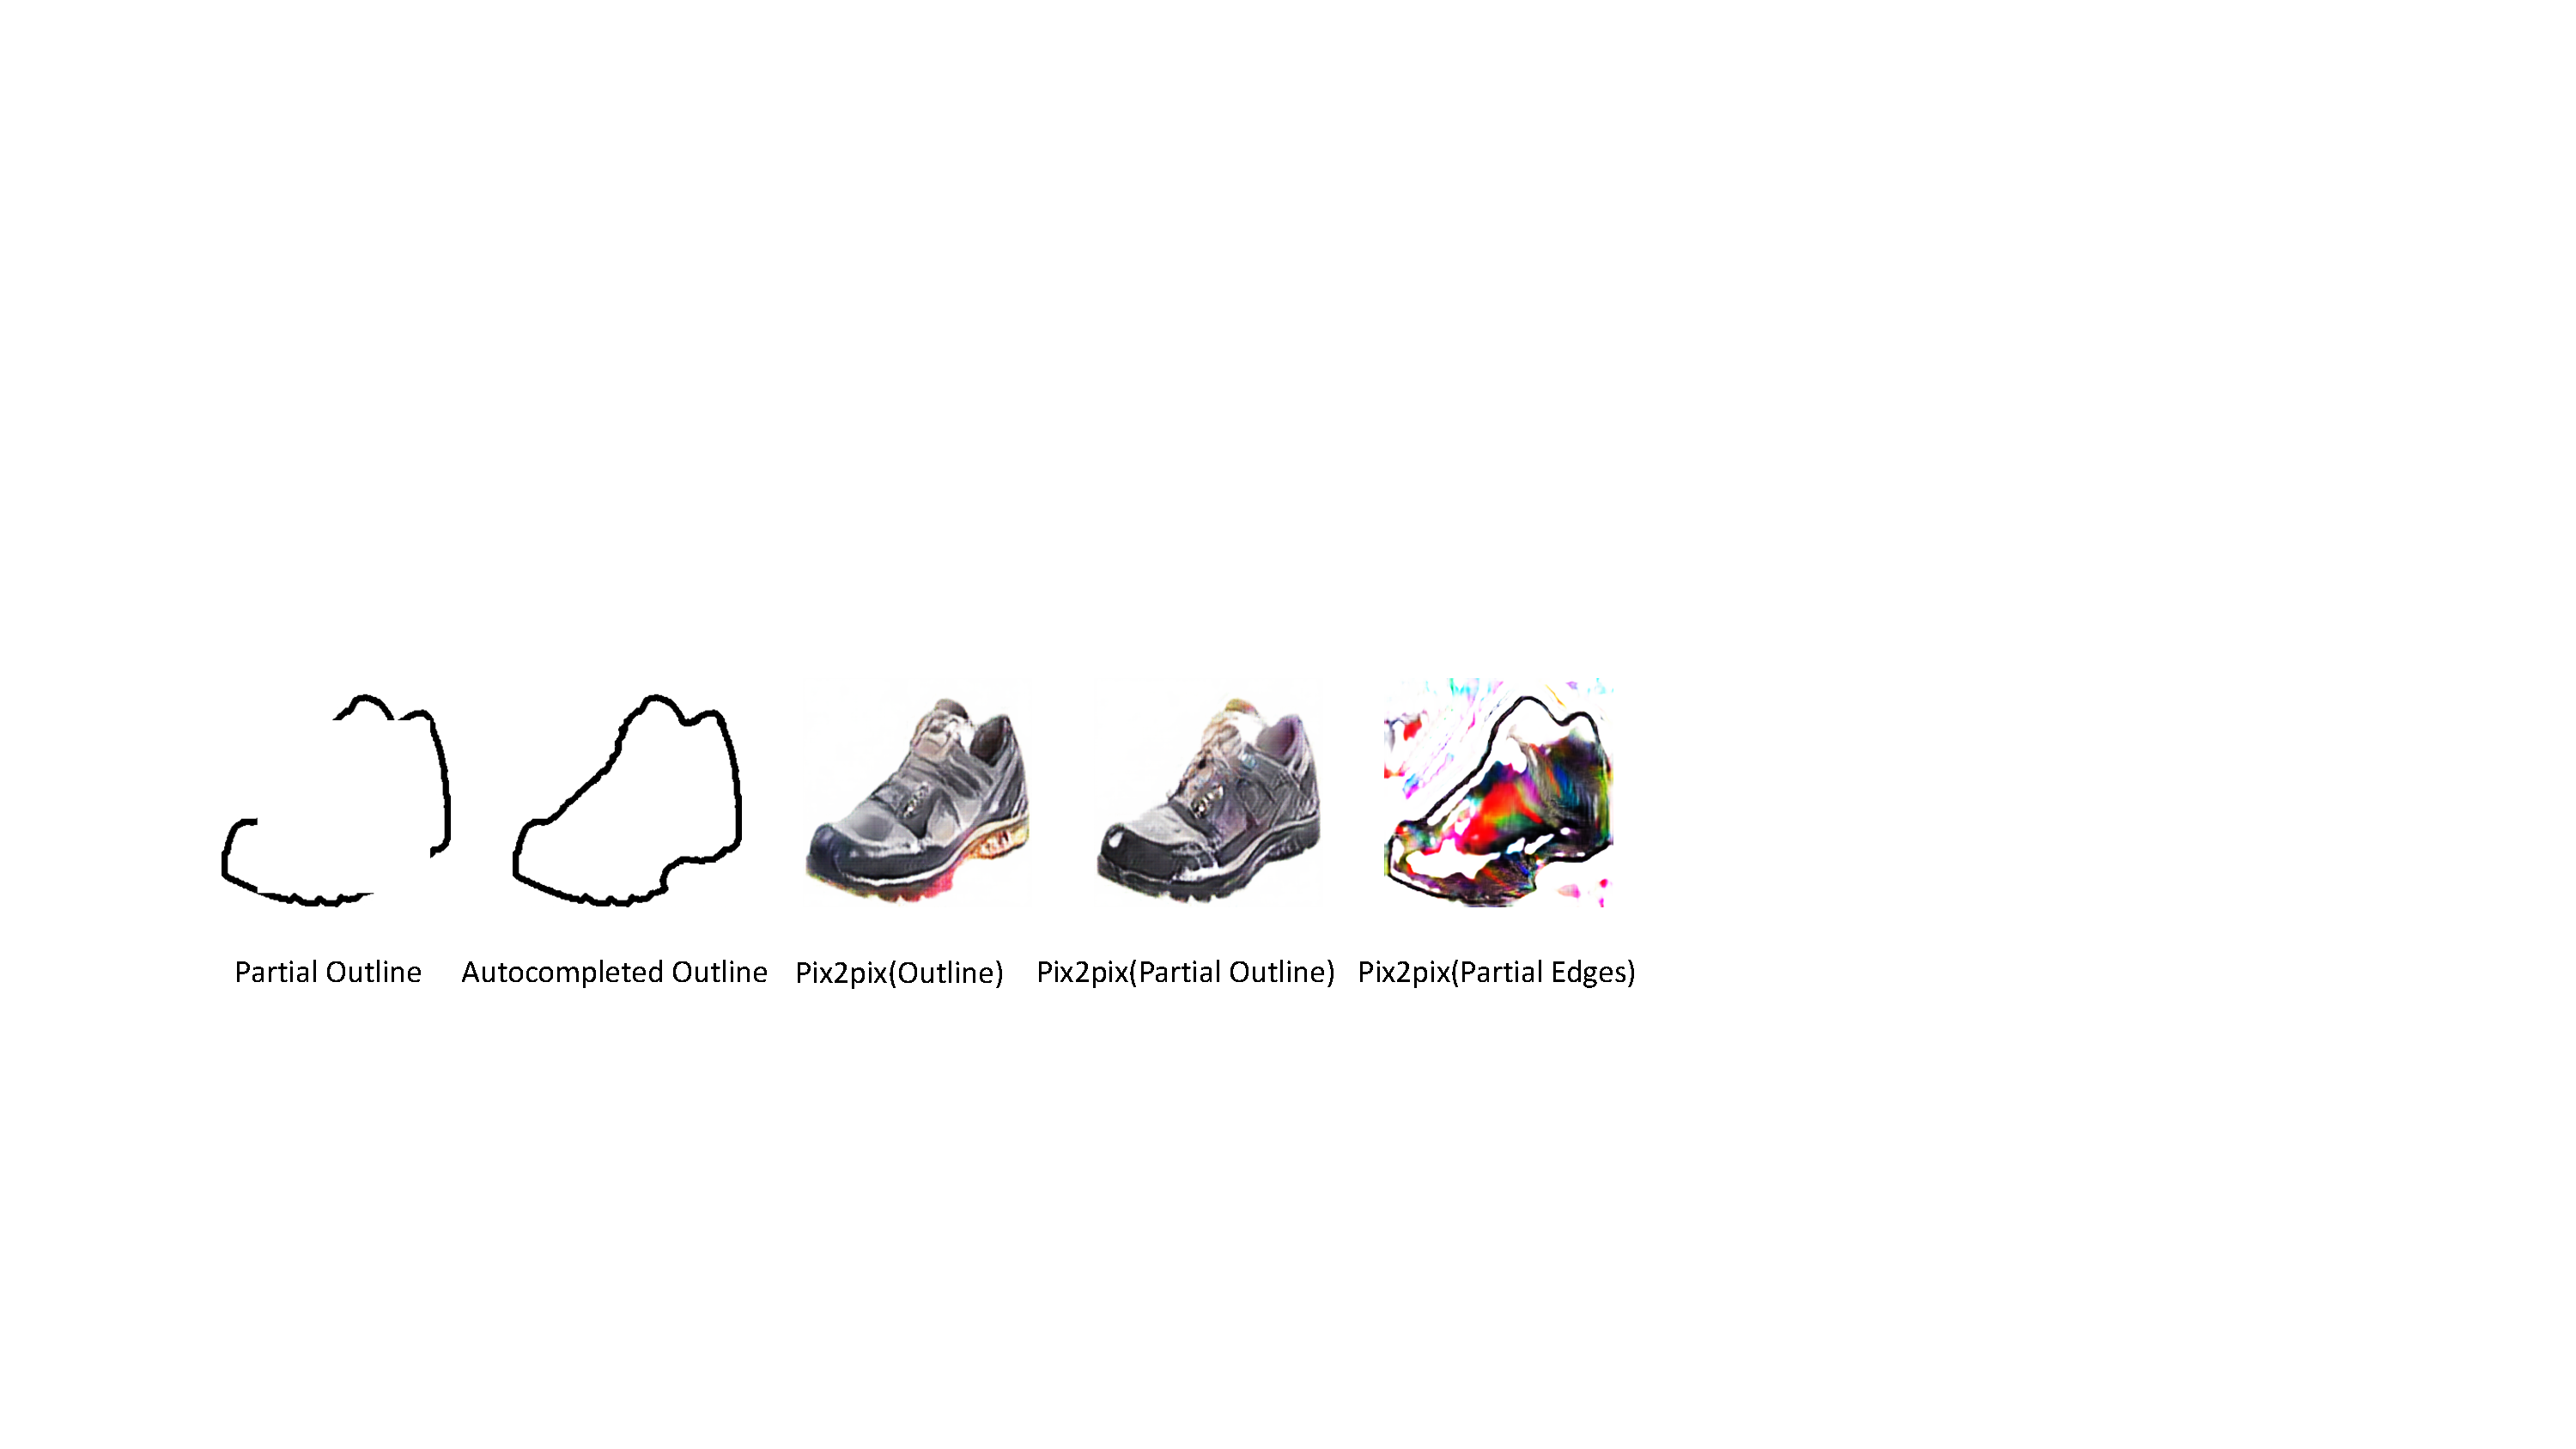
\includegraphics[width=1.\linewidth]{paper_images/outline_efficacy.pdf}
% %     \caption{\textbf{Shoe generation results}. Generating realistic images trained with partial sketches fails totally while images generated with partial outlines either directly or via an autocompleted image produces realistic results.
% %     % \ow{seems like this is missing 1. two generators, and 2. one generator. instead it seems more like an ablation study on our method, which is not the point. would be more impressive to show it matches 2 generators and 1 generator totally fails.}
% %     }
% %     \label{fig:shoe_outline_efficacy}
% %     \vspace{-2mm}
% % \end{figure*}

% % \subsection{Sparse Input Maps}
% % In order for a user guided system to be more interactive it must be able to generate images from sparse inputs and not wait for the user to provide the full sketch of the object. The sparse input can be obtained by either subsampling edges from the existing techniques used such as edgemaps \cite{isola2016image2image} or going towards even lesser supervision with outlines. In case of outlines, huge amounts of sparse data can be generated by occluding intermediate areas and generating sparse input maps. A simple approach for completing the real image from the partial sketch could be to directly train the generator to generate the real image from the partial outline or sketch. As we can see from \figref{fig:shoe_outline_efficacy} generating images from models trained on partial sketches fails to generate realistic images while using an outline either directly or via an autocomplete network leads to realistic results. 

% % In case of shoes the outline maps divulge a lot of information about the final generated result but simple general objects tend to have similar outlines and further a single network must be capable of generating multiple objects since it is the same shared task of image generation from outlines. Our experiments revealed as shown in \figref{fig:alg_comp} that naive conditioning techniques failed and necessitated the need for the gating network. The autocomplete network's output makes it easier to guide the user towards better image generation results and easier editing capabilities in the sketching interface. 


% % \paragraph{Autocomplete: Data Generation Procedure}
% % To simulate the effect of generating images from partial strokes, we take an input edge map or an outline map and occlude the map with a (white) square occluder at different scales to simulate the different quantities of the amount of strokes in the partial drawing. 

% % \noindent To explore the effectiveness of our soft-gating residual network, we test on a variety of settings.


% % \section{Experiments}
% % We present the details of a set of experiments performed and the corresponding results of the experiments which show the efficacy of our Gated Residual Blocks albeit being simple to implement.

% % \begin{itemize}[noitemsep]
% % \item {1-D unconditional modeling}
% % % We show that individual blocks in a residual network self-organize into modes in a simple 1-D distribution.
% % % \item {MNIST~\cite{XX} and FashionMNIST~\cite{XX} unconditional generation}
% % % We show that soft-gating can help improve generations in an InfoGAN setup.
% % \item {Outline$\rightarrow$Image class-conditional generation}
% % \item {Edges$\rightarrow$Handbags multimodal image generation}
% % \item {Disambiguating multiple disjoint tasks: Day$\rightarrow$Night and Cityscapes Label$\rightarrow$Image}
% % \end{itemize}



% % \subsection{1D incision experiment}

% % \begin{figure}[t]
% %     \centering
% %     %\addSubFigThird{Picture2}{ }{fig:1d_ground} 
% %     \addSubFigHalf{Picture33.png}{}{fig:1d_gen} 
% %     \addSubFigHalf{Picture3.png}{}{fig:1d_gen_rem}
% %     \caption{{\bf 1D Mixture of Gaussians experiment} \figref{fig:1d_gen} is the training distribution, and Generated Samples from the trained network. \figref{fig:1d_gen_rem} are the Generated Samples from the trained Generator with one of the blocks removed. \ow{make prettier}}
% %     \label{fig:onedexperiment}
% %     \vspace{-3mm}
% % \end{figure}

% % We first evaluate the effect of a gating network in the simple scenario of modeling a one dimensional mixture of Gaussians, comprised of five components. For this test, the generator and discriminator architectures consist of only residual blocks, where each residual block is composed of fully connected layers. Additional details are in the supplementary material. The generator is conditioned on a latent vector $z$. The generator is able to approximate the distribution, as seen in Fig.~\ref{fig:onedexperiment} (left). Removing a single residual block, in the spirit of~\cite{veit2016residual}, leads to the disappearance of a mode from the predicted distribution. Removal of another block leads to further removal of another mode, as seen in Fig.~\ref{fig:onedexperiment}  (mid, right). This experiment shows an encouraging result, suggesting that residual blocks decompose naturally into modeling parts of a distribution.

% % \paragraph{Incision Experiments} similar to \cite{veit2016residual} on the generator after the network is trained. More specifically, if a layer (say $i^{th}$) had to be skipped, we disable the $f_i(x)$ of the ith residual block and now the output of the $i^{th}$ residual block is $x$ in place of the usual $x+f_i(x)$ encountered during training. Some interesting observations could be made, for example removing some blocks corresponded to the vanishing of certain modes from the generated distribution once the incision was performed on the generator network. Another surprising observation was that the same mode vanished on the incision of certain different residual blocks. This experiment validated the hypothesis of \cite{veit2016residual} that residual networks behave like an ensemble of several shallower networks and also pointed out that another network could predict based on the condition which blocks to use and to skip other non-necessary blocks in the network for that particular condition.

% % \begin{figure}[t]
% %     \centering
% %     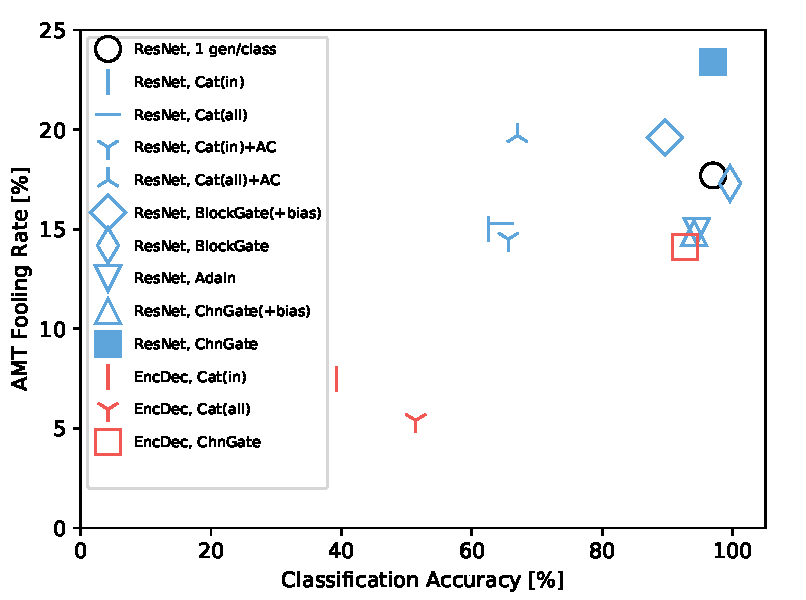
\includegraphics[width=\linewidth]{paper_images/gen_real_vs_acc.pdf}
% %     \caption{Generation realism vs accuracy}\label{fig:conditioning_amt}
% %     % \vspace{-4mm}
% % \end{figure}

% % \begin{figure*}[t]%[ht!]
% %     \centering
% %     % \addSubFigHalf{gated_G_act}{Generator}{fig:gen_act} \addSubFigHalf{gated_D_act}{Discriminator}{fig:dis_act} 
% %     % \caption{Activation of the various blocks in the Generator and Discriminator}
% %     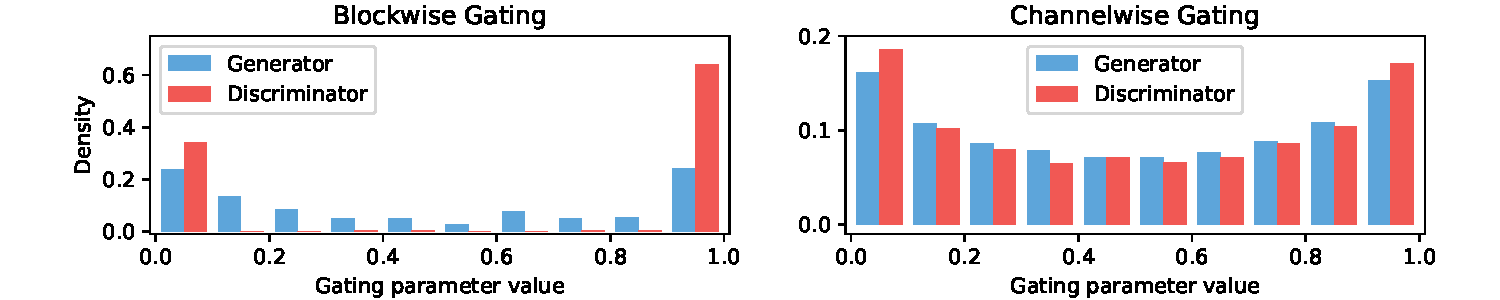
\includegraphics[width=\linewidth,trim={.7cm 0 .8cm 0},clip]{paper_images/alpha_hist.pdf}\caption{ {\bf Distribution of gating parameters.} We show the distribution of learned gating parameter $\alpha$ for {\bf (left)} blockwise and {\bf (right)} channelwise soft-gating. Values closer to 0,1 indicate that a residual block or channel is completely turned ``off" or ``on". In our best performing system, channelwise gating, the values are soft, but tend to be closer to the extremes.}
% %     \label{fig:alpha_dist}
% %     \vspace{-3mm}
% % \end{figure*}


% % \begin{figure*}
% %   \centering

% %   \begin{minipage}[b]{0.4\linewidth}
% %   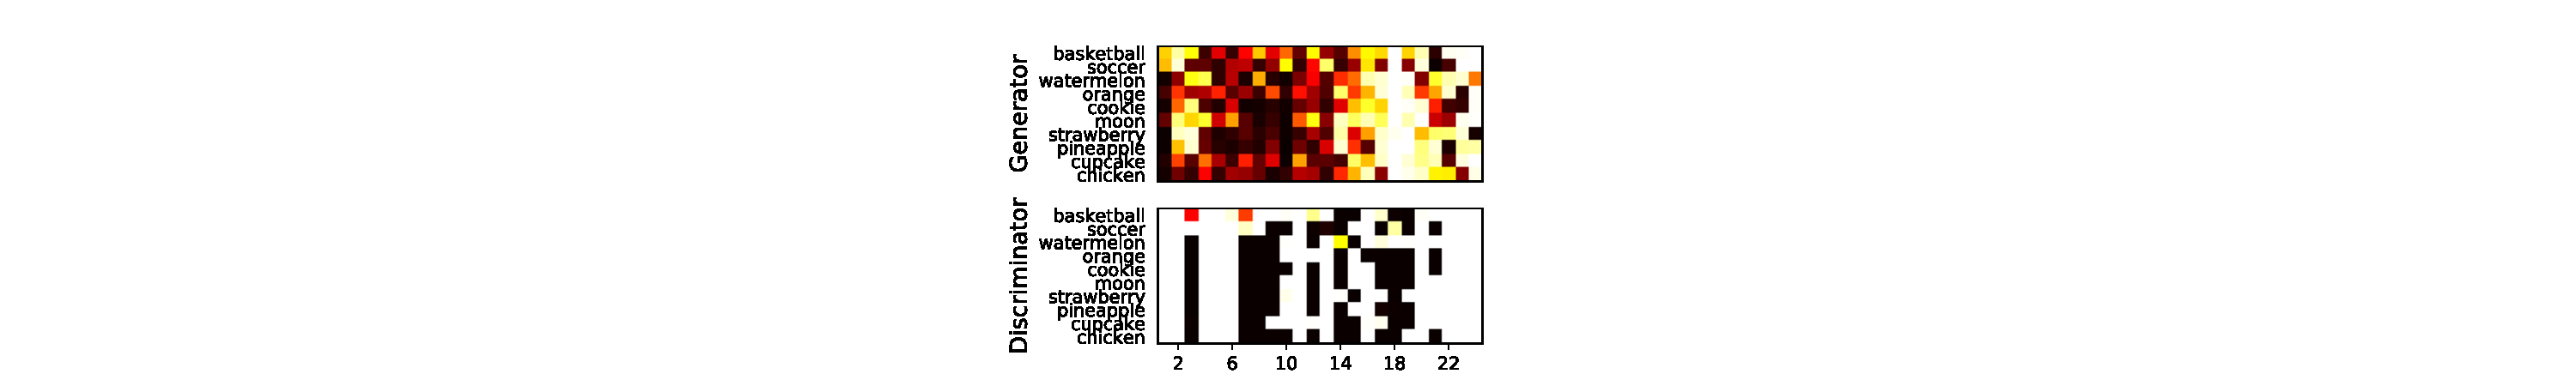
\includegraphics[width=\linewidth,trim={2cm 0 2cm 0},clip]{paper_images/alphas_block.pdf} 
% %   \end{minipage}
  
% %   \begin{minipage}[b]{0.45\linewidth}
% %   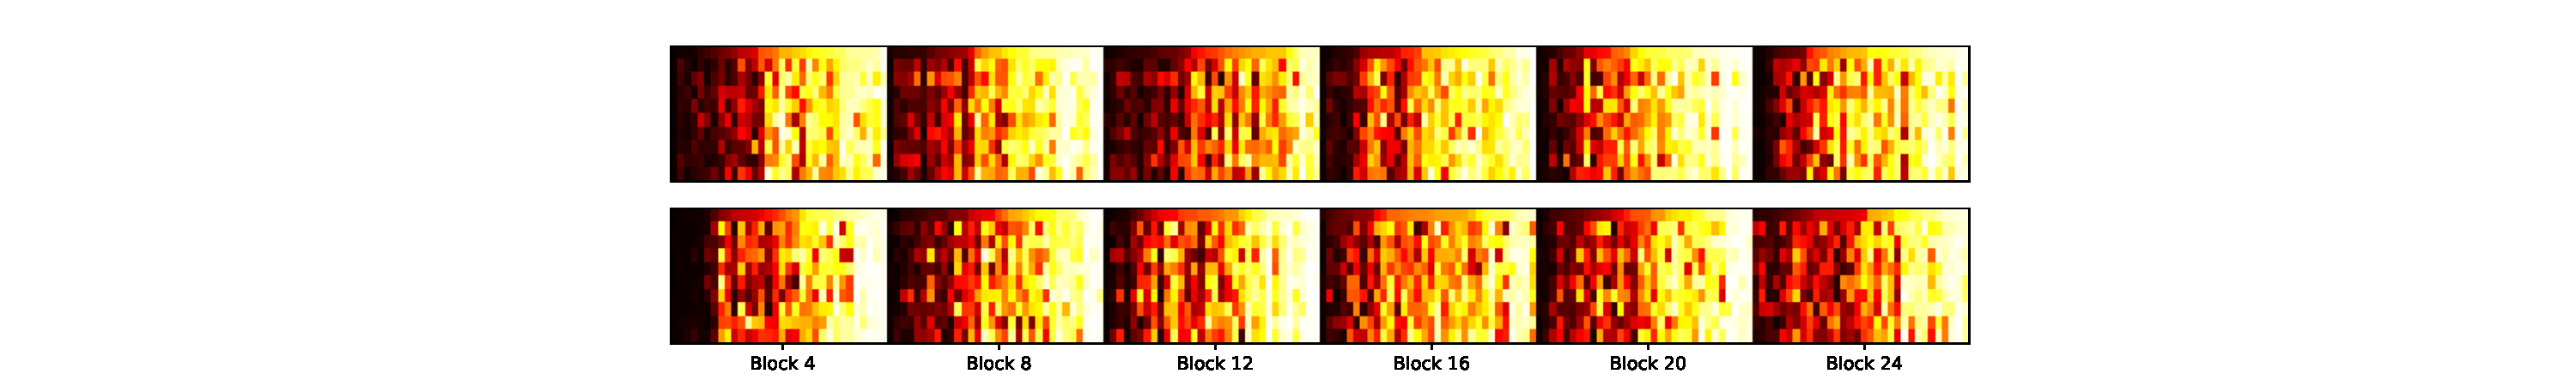
\includegraphics[width=\linewidth,trim={2cm 0 2cm 0},clip]{paper_images/alphas_chan.pdf} 
% %   \end{minipage}
  
% % %   \vspace{-4mm}
% %   \caption{\small \textbf{(Left)}  \textbf{(Right)} 
% %   }
% % %   \vspace{-5mm}
% %   \label{fig:alphas}
% % \end{figure*}

% % \paragraph{Network Architecture}
% % \rz{shorten this into a few sentences for each net, so reader knows what we tested later, and point to suppmat where the tables can go}

% % \subsection{Outline$\rightarrow$Image}
% \subsection{Class-conditional image translation}

% \noindent We further investigate the effect of soft-gating in image modeling scenarios on multiclass generation. We first describe our dataset (new) which contains pairs of sparse scribbles and images.

% \vspace{2mm} \noindent \textbf{Dataset} Previous work~\cite{isola2016image2image,sangkloy2017scribbler,zhu2017unpaired,wang2017high} trained edge-to-image translation networks, which are then repurposed into a sketch-to-image translation machine, sometimes gaining unexpected popularity\footnote{Edges to cats demo: https://affinelayer.com/pixsrv/}. We collect 200 images (150 train, 50 test) for each of 10 classes -- basketball, chicken, cookie, cupcake, moon, orange, soccer, strawberry,  watermelon and pineapple -- and obtain rough outlines for each image. %using Adobe Photoshop
% % Unlike previous work on scribble-to-image translation \cite{isola2016image2image,zhu2017unpaired,wang2017high},
% Our outlines contain significantly less edge information. This makes the multitask generation problem more challenging -- for example, the same circular outline can draw a basketball, soccerball, or watermelon. A network must effectively integrate class information to be successful in this setting.
% % , as the internal features must be learned by the network, and the same outline can generate substantially different images conditioned on different classes.
% % , as seen in Fig.~\ref{fig:teaser}.
% %The task involves multiple different objects of high realism when the input is very similar for the various classes several of them being exactly same(in the case of circular objects where the input scribble is an identical scribble for all circular classes). 

% \vspace{2mm} \noindent \textbf{Network Architecture} Our preliminary experiments, using the architecture based on MUNIT~\cite{huang2018multimodal} did not succeed for this task. The architecture, which we refer to as \textbf{Encoder-Decoder}, is comprised of 3 \texttt{conv} layers, 8 residual blocks, and 3 \texttt{up-conv} layers. The residual blocks have 256 channels. We deepen the network, based on the principle that deeper networks have more valid disjoint, partially shared, paths~\cite{veit2016residual}, and add 24 residual blocks. To enable the larger number of residual blocks, we drastically reduce the width to 32 channels for every layer. We refer to this network as \textbf{SkinnyResNet}. Additionally, modifying the downsampling and upsampling blocks to be residual improved results, and also enables us to apply gating to {\em all} blocks. % , including the upsampling and downsampling residual blocks, improves the quality of generations. Additionally, we discover that even having few blocks  Details about the architecture can be found in the supplementary. \eli{explain why skinny.}
% When gating is used, the gate prediction network, $\mathcal{F}$ in Fig.~\ref{fig:arch-inj} (mid-right, right) is also designed using residual blocks. Additional architectue details are in the supplementary material. 
% We systematically test methods for injecting class information, as described in Sec.~\ref{sec:methods}. \begin{itemize}[noitemsep]
% \item{\bf Per-class}: a single generator for each category; this is the only test setting with \textit{multiple} networks, all others train a single network
% \item{\bf Concat (In)}: naive concatenation, input layer only
% \item{\bf Concat (All)}: naive concatenation, all layers
% \item{\bf Concat (In)+Aux-Class}: we add an auxiliary classifier, both for input-only and all layers settings
% \item{\bf BlockGate(+Bias), BlockGate}: block-wise soft-gating, with and without a bias parameter
% \item{\bf AdaIn}: Adaptive instance normalization
% \item{\bf ChannelGate(+Bias), ChannelGate}: channel-wise soft-gating, with and without a bias parameter
% \end{itemize}





% % \begin{figure*}[t]
% % \centering
% % \begin{tabular}{*{3}{c@{\hspace{3px}}}}
% % \textbf{Blockwise Gating} & \textbf{Channelwise Gating} \vspace{-1mm} & \\
% % 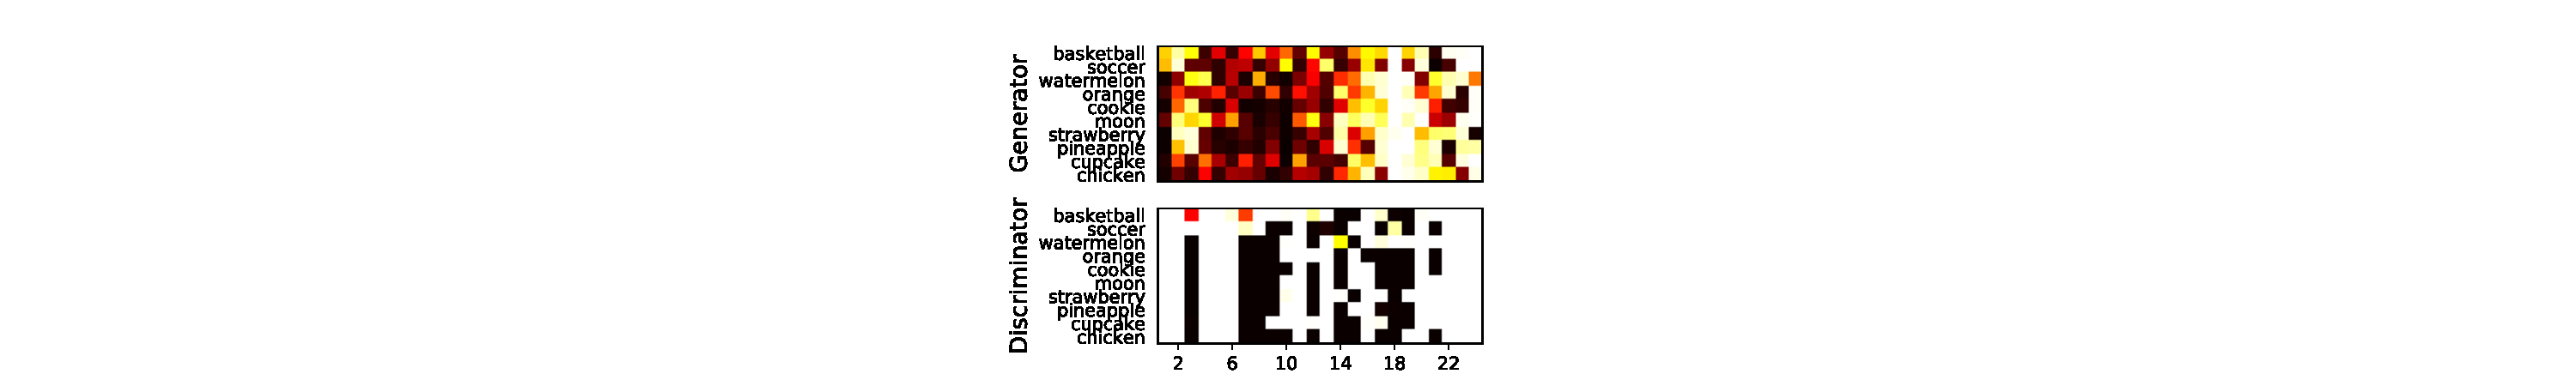
\includegraphics[height=3.35cm,trim={.15cm 0 0 .4cm}, clip]{paper_images/alphas_block.pdf} &
% % 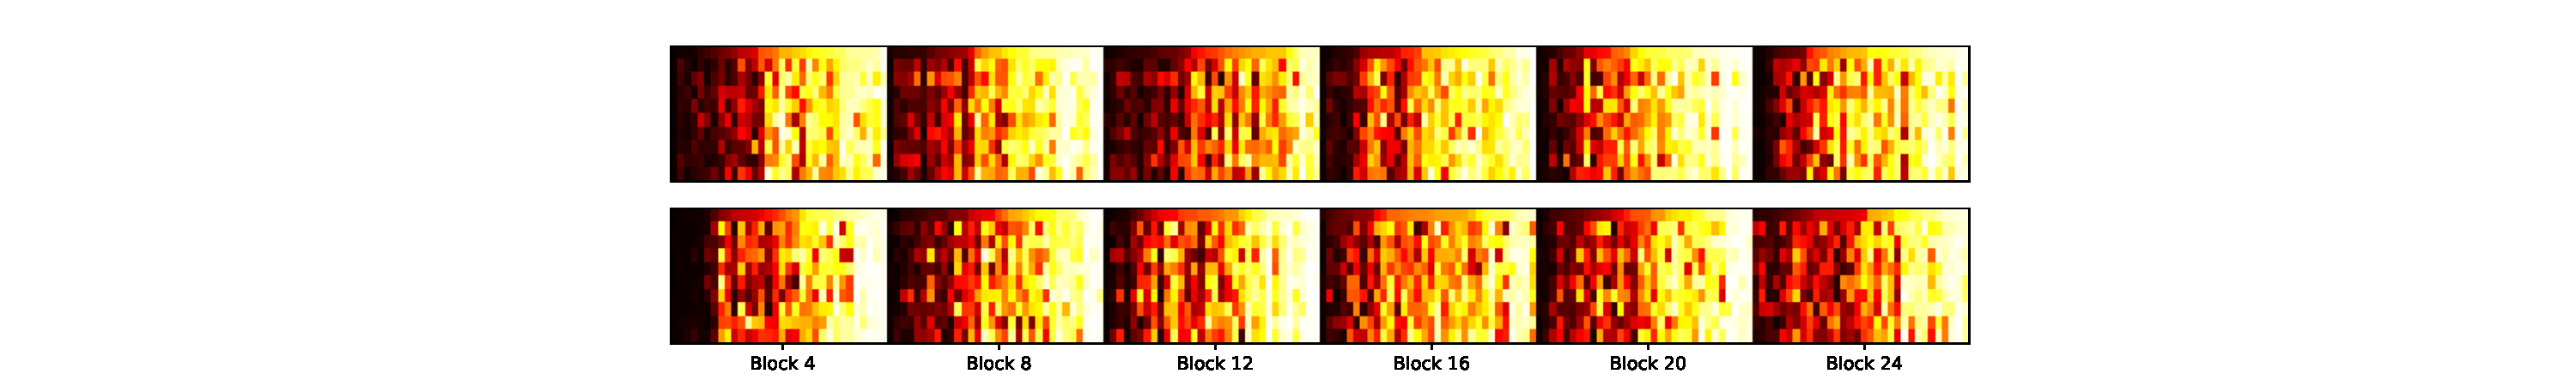
\includegraphics[height=3.35cm,trim={0 0 0 .4cm}, clip]{paper_images/alphas_chan.pdf} & 
% % 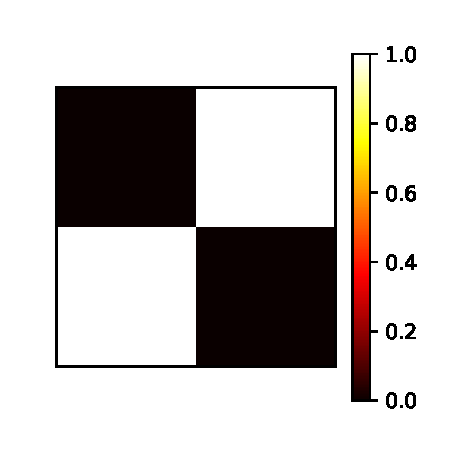
\includegraphics[height=3.35cm,trim={5.8cm 0 .2cm .4cm}, clip]{paper_images/alpha_legend.pdf}
% % \\
% % \end{tabular}
% % \vspace{-2mm}
% % \caption{\label{fig:alpha_heat}
% % \textbf{Learned gating parameters.} We show the soft-gating parameters for {\bf (left)} blockwise and {\bf (right)} channelwise gating for the {\bf (top)} generator and {\bf (bot)} discriminator. Black indicates
% % % $\alpha=0$, or
% % completely off, and white indicates
% % % $\alpha=1$, or 
% % completely on. For channelwise, a subset (every 4th) of blocks is shown. Within each block, channels are sorted in ascending order of the first category. The nonuniformity of each columns indicates that different channels are used more heavily for different classes.
% % \vspace{-3mm}
% % }
% % \vspace{-2mm}
% % \end{figure*}




% % with each residual block consisting of 1D convolution layers. 

% \begin{figure*}[h]
%     \centering
%     \includegraphics[width=.9\linewidth]{paper_images/cond_comp2.pdf}
%     \caption{{\bf Conditioning injection comparison.} We show results across methods on the outline$\rightarrow$image task using the \textbf{SkinnyResNet} architecture. Naive Concatenation \textbf{Concat} often confuses classes, such as oranges and basketballs, while gating mechanisms such as the \textbf{ChannelGate} method succeed. The gating method also improves results for the \textbf{EncoderDecoder} architecture. \label{fig:alg_comp} }
%     \vspace{-4mm}
% \end{figure*}


% % The incision experiments as performed by \cite{veit2016residual} showed that deeper networks have more  valid paths of computation. Our incision experiments on the 1D Mixture of Gaussians setting also demonstrated the effectiveness of having deeper residual networks with lesser number of neurons in each block. We therefore design a network architecture which doesn't change the number of channels even in the case where the spatial resolution changes since the gating is applied to all the blocks including the downsampling and upsampling residual blocks and the hypothesis is that the gating mechanism would work best if all the blocks had similar number of modulations per block.


% \vspace{2mm} \noindent \textbf{Evaluation Metrics} We evaluate the results on two axes: adherence to conditioning and realism. We first test the conditioning adherence -- whether the network generates an image of the correct class. Off-the-shelf networks have been previously used to evaluate colorizations~\cite{zhang2016colorful}, street scenes~\cite{isola2016image2image, wang2017high}, and ImageNet generations~\cite{salimans2016improved}. We take a similar approach and fine-tune a pretrained InceptionV3 network~\cite{szegedy2016rethinking} for our 10 classes. The generations are then tested with this network for classification accuracy.
% % The class specific generations from the testset were passed through the finetuned network and the classifications were used to judge the class specific purity of the generations.

% To judge the generation quality, we perform a ``Visual Turing test" using Amazon Mechanical Turk (AMT). Turkers are shown a real image, followed by a generated image, or vice versa, and asked to identify the fake. An algorithm which generates a realistic image will ``fool" Turkers into choosing the incorrect image. We use the implementation from~\cite{zhang2016colorful}. We show quantitative results in Fig.~\ref{fig:acc_vs_real} and qualitative examples in Fig.~\ref{fig:alg_comp}.

% \vspace{2mm} \noindent \textbf{Does naive concatenation effectively inject conditioning?} In Fig.~\ref{fig:alg_comp}, we show a selected example from each of the 10 classes. The per-class baseline trivially adheres to the conditioning, as each class gets to have its own network. However, when a single network is trained to generate all classes, naive concatenation is unable to successfully inject class information, for either network and for either type of concatenation. For the \textbf{EncoderDecoder} network, basketballs, oranges, cupcakes, pineapples, and fried chicken are all confused with each other. For the \textbf{SkinnyResNet} network, oranges are generated instead of basketballs, and pineapples and fried chicken drumsticks are confused. As seen in Fig.~\ref{fig:acc_vs_real}, classification accuracy is slightly higher when concatenating all layers ($64.5\%$) versus only the input layer ($62.6\%$), but is low for both.
% % As evident from \figref{fig:alg_comp} for some classes naive concatenation helps in generating appealing images but for some classes it either fails to generate images from the right class or generates unrealistic images from that class.
% % No, point to Figure 9 (qualitative grid) \& Figure 10 (the plot)

% % \paragraph{Does gating produce accurate and realistic conditional generations?} The gating mechanisms succeeds in generating realistic images from each class while also preserving the class conditioning appropriately. As evident from the comparisons of generations in \figref{fig:alg_comp} and the metrics reported in \figref{fig:conditioning_amt} the channel wise multiplication produces the most visually appealing results amongst the various gating mechanisms.
% % Yes, point to Figure 9 results. Also analyze which variation is the best

% \vspace{2mm} \noindent \textbf{Does gating effectively inject conditioning?} Using the proposed soft-gating, on the other hand, leads to successful generations. We test variants of soft-gating on the \textbf{SkinnyResNet}, and accuracy is dramatically improved, between $89.6\%$ to $99.6\%$, comparable to using a single generator per class ($97.0\%$).
% % \pd{Two variants of gating provide accuracy better than per-class generator.}
% Among the gating mechanisms, we find that channel-wise multiplication
% % (on both generator and discriminator)
% generates the most realistic images, achieving an AMT fooling rate of $23.4\%$. Interestingly, the fooling rate is higher than the per-class generator of $17.7\%$. Qualitatively, we notice that per-class generators sometimes exhibits artifacts in the background, as seen in the generation of ``moon". We hypothesize with the correct conditioning mechanism, the single generator across multiple classes has the benefit of seeing more training data and finding common elements across classes, such as clean, white backgrounds.
% % \pd{it can be confusing also. is it a good justification?}
% % The classification accuracy of an Inception network finetuned on our dataset demonstrates the purity of the generations corresponding to the correct class using the gating mechanism. 

% % As seen in \figref{fig:alg_comp}, all of the various gating mechanisms and the baselines are able to generate images of high quality and realism from some classes but most of the baselines fail in some classes, often mixing visual features from wrong classes. 




% % \begin{table*}[t]
% %   \floatsetup{floatrowsep=qquad, captionskip=4pt}
% %   \centering
% %     \begin{floatrow}[2]
% %     \ffigbox[\FBwidth]{
% %     \scalebox{0.95} {
% %         \begin{tabular}{l c}
% %         % \hline
% %         \toprule
% %         \textbf{Model} & \textbf{LPIPS Distance} \\ \midrule
% %         Random Real Images & $0.3665 \pm 0.0053$ \\ \midrule
% %         BicycleGAN~\cite{zhu2017toward} & $0.1374 \pm 0.0005$  \\ \midrule
% %         Concat(In) &  $0.0432 \pm 0.0002$ \\
% %         Concat(All) & $0.0159 \pm 0.0004$ \\ \cdashline{1-2}
% %         ChannelGate [Ours] & $0.0964 \pm 0.0003$  \\
% %         \bottomrule %inserts single line
% %         \end{tabular}}}
% %         {\caption{\label{table:infogan_lpips} {\bf Edges$\rightarrow$Handbags Diversity.} LPIPSv0.1~\cite{zhang2018unreasonable} distance between randomly generated handbags, given the same edge map, as proposed in~\cite{zhu2016generative}. Given the same architecture, gating achieves higher diversity than concatenation.}}
% %         \ffigbox[\FBwidth]{
% %         \scalebox{0.95} {
% %         \begin{tabular}{l c c c} % 
% %         % \begin{tabular}{p{6cm}c{1.8cm}c{1.8cm}c{1.8cm}} % centered columns (4 columns)
% %         \toprule
% %         \multirow{2}{*}{\textbf{Model}} & \textbf{Per-pixel} &  \textbf{Per-class } & \textbf{Class} \\
% %         & \textbf{Acc} &  \textbf{Acc} & \textbf{IOU} \\ \midrule
% %         Pix2pix \cite{isola2016image2image} & 0.660  & 0.23 & 0.17 \\ \midrule
% %         EncDec, Concat(All) & 0.600 & 0.16 & 0.15 \\ \cdashline{1-4}
% %         SkinnyResNet, Cat(All) & 0.602 & 0.18 & 0.16 \\
% %         SkinnyResNet, Cat(All)+Aux-Class & 0.675 & 0.20 & 0.16 \\ \cdashline{1-4}
% %         SkinnyResNet, ChannelGate [Ours] & 0.684 & 0.23 & 0.18 \\ \bottomrule
% %         % \bottomrule %inserts single line
% %         \end{tabular}}}{
% %         \caption{ {\bf Cityscapes generation accuracy}. We evaluate the accuracy of Cityscapes Label$\rightarrow$Image generation results, as part of the multitask test. The network is also trained for an unrelated Day$\rightarrow$Night task. A pre-trained segmentation network, as used in~\cite{isola2016image2image} evaluates the synthesized results. Gating achieves higher results than concatenation, as well as single-task pix2pix~\cite{isola2016image2image}. }
% %         \label{label:me}}
    
% %     \vspace{-3mm}
% %   \end{floatrow}
% % %  \vspace{-2mm}
% % %   \label{fig:real_vs_div}
% % \end{table*}


% % \begin{figure}
% %     \centering
% %     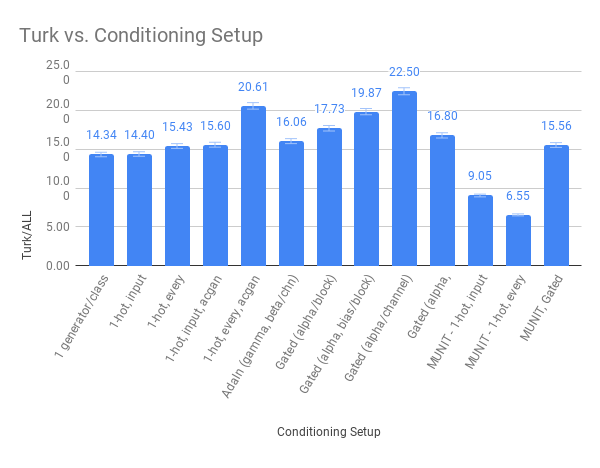
\includegraphics[width=\linewidth]{conditioning_amt.png}
% %     \caption{AMT studies of the various gating techniques on the scribble dataset}\label{fig:conditioning_amt}
% %     \vspace{-4mm}
% % \end{figure}



% \vspace{2mm} \noindent \textbf{Is gating effective across architectures?} 
% % We evaluate the following architectures on the outlines-to-images task. 
% % We first evaluate our \todo{SkinnyResNet} with a more traditional encoder-decoder architecture. 
% % We use the architecture proposed in MUNIT~\cite{huang2018multimodal} which consists of an encoder followed by a set of residual blocks with a decoder at the end.
% As seen in Fig.~\ref{fig:acc_vs_real}, using channelwise gating instead of naive concatenation improves performance both accuracy and realism \textit{across} architectures. For example, for the \textbf{EncoderDecoder} architecture, gating enables successful generation of the pineapple.
% % In this case, we apply the gating to this architecture only on the bottleneck residual blocks.
% % As evident from \figref{fig:alg_comp} although the network learns to disentangle the various classes, the generation quality reduces from the skinny resnet architecture where all the layers are gated.
% Both quantitatively and qualitatively, results are better for our proposed \textbf{SkinnyResNet} architecture.

% % Yes, works for both skinny resnet \& enc-dec.

% \vspace{2mm} \noindent \textbf{Do the generations generalize to unusual outlines?} The training images consist of the outlines corresponding to the geometry of each class. However, an interesting test scenario is whether the technique generalizes to unseen shape and class combinations. In \figref{fig:teaser}, we show that an input circle not only produces circular objects, such as a basketball, watermelon, and cookie, but also noncircular objects such as strawberry, pineapple, and cupcake. Note that both the pineapple crown and bottom are generated, even without any structural indication of these parts in the outline.

% \vspace{2mm} \noindent \textbf{How are the gating coefficients distributed?} In Fig.~\ref{fig:alpha_heat}, we show the predicted block and channel gating parameters. For blockwise gating, the coefficients of discriminator are almost completely binary. For channelwise gating, the values are softer. The values tend to be closer to the extremes (0 or 1) than the middle (0.5). Please see the supplementary material for further analysis on the distribution of values. In general, the gating parameters exhibit correlation, indicating that blocks and channels are typically used across categories. However, some blocks or channels do specialize to certain categories, as indicated by the nonuniformity of columns in the plot.
% % \pd{any insights from this would be good. also, can we compare these two since channelwise has way more alphas than blockwise.}
% % An interesting observation of the gating coefficients in the case of the block wise gating mechanism, as demonstrated in \figref{fig:gated_block_act} for different classes different sets of blocks were activated and some blocks were totally deactivated for some classes. The switching on and off of various blocks without even adding a sparsity constraint was better defined in the case of the discriminator.


% % \begin{figure*}[h]
% %     \centering
% %     \includegraphics[width=.94\linewidth]{paper_images/cond_comp2.pdf}
% %     \caption{{\bf Algorithm Comparison} \label{fig:alg_comp} }
% %     \vspace{-4mm}
% % \end{figure*}



% % \begin{figure}
% %     \centering
% %     \includegraphics[width=\linewidth]{paper_images/cond_comp.pdf}
% %     \caption{Algorithm Comparison}\label{fig:conditioning_amt}
% % \end{figure}

% % In the widely popular image conditioned generative models introduced in Pix2pix by \cite{isola2016image2image} although the results are brilliant, it had the inherent problem of only being applicable to a particular task such as different networks had to be trained for edges to shoes and edges to handbags, although StarGAN \cite{choi2017stargan} mitigated some of the problems but it was only applicable for relatively minute transformations such as changing the characteristics of the face.

% % To analyze properly the task of multi-class generations in the image conditioned setting we introduce a new task of generating class conditioned realistic images from very rough scribbles. We start off with 3 classes, namely: pizza, strawberry and oranges. A simple pix2pix network fails to identify the different classes and starts injecting weird textures such as pizza on orange or strawberry on pizza as depicted in the results from pix2pix on this task in \figref{fig:scribble_pix2pix}. 

% % In the conditional setting for the generator, the main block only receives the input scribble and the gate selection block receives the class condition and predicts the $aplha^i$s for the gated residual blocks. The discriminator on the other hand is composed of a main network consisting of gated residual blocks which is oblivious to the class conditioning and a gate selection network which predicts the $aplha^i$s for the main network of the discriminator. The main network also receives the input scribble alongside the generated/real image to predict how real/fake an image is based on the alpha weightings of its gated residual blocks. The network is able to disentangle the class conditioning although none of the main networks of the generator/ discriminator are aware of the class conditioning, the class information only being input to the gate selection network which has to modulate the weights of the respective networks' gated residual blocks. The results of the model are depicted in \figref{fig:scribble_grb} whereby we can clearly see that the network has been able to disentangle the class conditioning and generate textures appropriate for the right class.


% % \subsection{Comparison to other forms of conditioning in Resblock :}
% % Conditional Batch Normalization, FiLM and Adaptive Instance Normalization are the techniques which are the most closely related to our methodology. All of these have the benefit of being applicable even without the presence of residual blocks in the architecture. So an exhaustive comparison with all of these methods along with our form of conditioning on the residual blocks is a valid set of experimentation and has to be done to make the paper complete.

% % \subsection{Infogan Variations(pix2pix):}


% % \begin{table}[ht]
% % \caption{Evaluation on Edges to Handbags diverse generations. Diversity using LPIPS metric \cite{zhang2018unreasonable}} % title of Table
% % \small
% % \centering % used for centering table
% % % \begin{tabular}{|c|c|c|c|} % centered columns (4 columns)
% % \begin{tabular}{p{3cm}p{3cm}} % centered columns (4 columns)
% % % \hline
% % \toprule
% % \textbf{Model} & \textbf{LPIPS Distance} \\%heading
% % \midrule
% % BicycleGAN \cite{zhu2017toward} & $0.1374 \pm 0.0005$  \\ % inserting body of the table
% % \midrule
% % Ours(Gated) & $0.0964 \pm 0.0003$  \\
% % \midrule
% % Concat(Input) &  $0.0432 \pm 0.0002$ \\
% % \midrule
% % Concat(All Layers) & $0.0159 \pm 0.0004$ \\
% % \midrule
% % Random Real Images & $0.3665 \pm 0.0053$ \\
% % \bottomrule %inserts single line
% % \end{tabular}
% % \label{table:infogan_lpips} % is used to refer this table in the text
% % \end{table}

% % \begin{figure*}[t]%[ht!]
% % \centering
% % \begin{tabular}{*{5}{c@{\hspace{3px}}}}
% %     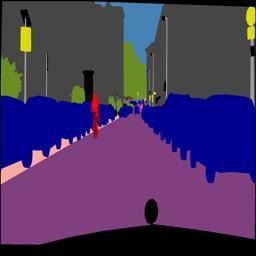
\includegraphics[width=.18\linewidth]{channel_gated/cityscapes_95_real_A} &
% %     \includegraphics[width=.18\linewidth]{munit_baseline_all/cityscapes_95_fake_B} &
% %     \includegraphics[width=.18\linewidth]{our_baseline_all/cityscapes_95_fake_B} & 
% %     \includegraphics[width=.18\linewidth]{acgan_baseline_all/cityscapes_95_fake_B}&
% %     \includegraphics[width=.18\linewidth]{channel_gated/cityscapes_95_fake_B} \\
    
% %     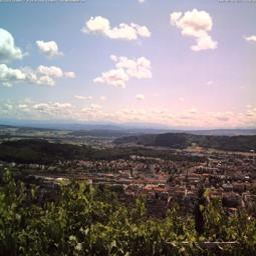
\includegraphics[width=.18\linewidth]{final_images/channel_gated/night2day_35_3106_to_3109_real_A.jpg} &
% %     \includegraphics[width=.18\linewidth]{munit_baseline_all/night2day_35_3106_to_3109_fake_B} &
% %     \includegraphics[width=.18\linewidth]{our_baseline_all/night2day_35_3106_to_3109_fake_B} &
% %     \includegraphics[width=.18\linewidth]{acgan_baseline_all/night2day_35_3106_to_3109_fake_B} & 
% %     \includegraphics[width=.18\linewidth]{channel_gated/night2day_35_3106_to_3109_fake_B}\\
    
% %     \begin{subfigure}[t]{.18\linewidth}\caption{\small Input}\label{fig:daynightinput}\end{subfigure} &
% %     \begin{subfigure}[t]{.18\linewidth}\caption{\small Enc-Dec Concat (All)}\label{fig:daynightinput}\end{subfigure} &
% %     \begin{subfigure}[t]{.18\linewidth}\caption{\small Concat (All)}\label{fig:daynightinput}\end{subfigure} &
% %     \begin{subfigure}[t]{.18\linewidth}\caption{\small Concat(All)+Aux-Class}\label{fig:daynightinput}\end{subfigure} &
% %     \begin{subfigure}[t]{.18\linewidth}\caption{\small Ours}\label{fig:daynightinput}\end{subfigure}\\
% % \end{tabular}
% %     % \addSubFigEighth{channel_gated/cityscapes_95_real_A}{input}{fig:city_input} 
% %     % \addSubFigEighth{channel_gated/cityscapes_95_fake_B}{Ours}{fig:city_ours} 
% %     % \addSubFigEighth{munit_baseline_all/cityscapes_95_fake_B}{MUNIT Conditioning all layers}{fig:city_munit}
% %     % \addSubFigEighth{our_baseline_all/cityscapes_95_fake_B}{Our Architecture Conditioning all layers}{fig:bag_3}
% %     % \addSubFigEighth{acgan_baseline_all/cityscapes_95_fake_B}{ACAN (our Architecture Conditioning all layers) }{fig:bag_3}
% %     % \caption{Various Methods for Cityscapes for Multi-Task Experiment}
% %     % \label{fig:multi-task_cityscapes}
% %     % \vspace{-3mm}
% %     % \addSubFigEighth{channel_gated/night2day_58_5018_to_5000_real_A}{input}{fig:city_input} 
% %     % \addSubFigEighth{channel_gated/night2day_58_5018_to_5000_fake_B}{Ours}{fig:city_ours} 
% %     % \addSubFigEighth{munit_baseline_all/night2day_58_5018_to_5000_fake_B}{MUNIT Conditioning all layers}{fig:city_munit}
% %     % \addSubFigEighth{our_baseline_all/night2day_58_5018_to_5000_fake_B}{Our Architecture Conditioning all layers}{fig:bag_3}
% %     % \addSubFigEighth{acgan_baseline_all/night2day_58_5018_to_5000_fake_B}{ACAN (our Architecture Conditioning all layers) }{fig:bag_3}
% %     \caption{Results on the multi-task generation problem with Segmentation2Cityscapes and Day2Night. \ow{seems like this is missing 1. two generators, and 2. one generator. instead it seems more like an ablation study on our method, which is not the point. would be more impressive to show it matches 2 generators and 1 generator totally fails.}}
% %     \label{fig:multi-task_day2night}
% %     \vspace{-3mm}
% % \end{figure*}


% % \begin{table}[ht]
% % \caption{Evaluation on Cityscapes for Multi-Task scenario. A pre-trained segmentation network~\cite{} performs a semantic segmentation on generated images, and the result is compared to the ground truth.} % title of Table
% % \small
% % \centering % used for centering table
% % % \begin{tabular}{|c|c|c|c|} % centered columns (4 columns)
% % \begin{tabular}{p{3cm}p{1cm}p{1cm}p{1cm}} % centered columns (4 columns)
% % % \hline
% % \toprule
% % \textbf{Model} & \textbf{Per-pixel acc.} &  \textbf{Per-class acc.} & \textbf{Class IOU} \\%heading
% % \midrule
% % Pix2pix \cite{isola2016image2image} & 66 \%  & 0.23 & 0.17 \\ % inserting body of the table
% % \midrule
% % Ours(Channel-Gate) & 68.4 \%  & 0.23 & 0.18 \\
% % \midrule
% % Concat(All),Aux-class & 67.5 \% & 0.2 & 0.16 \\
% % \midrule
% % Concat(All) & 60.2 \% & 0.18 & 0.16 \\
% % \midrule
% % Enc-Dec, Concat(All) & 60 \% & 0.16 & 0.15 \\
% % \bottomrule %inserts single line
% % \end{tabular}
% % \label{table:1d_G} % is used to refer this table in the text
% % \end{table}

% % \vspace{-1mm}
% % \subsection{Multi-Task Generation}
% % We also evaluate two previously shown image-to-image translation tasks -- segmentation$\rightarrow$street scene, and day $\rightarrow$ night -- using the {\em same} network. 
% % %Since our network is robust enough to be able to generate images conditioned on class and modulation of which blocks to use, it can further be used to generate images which are different in tasks such as the same network
% % As shown in \figref{fig:multi-task_day2night}, our model (ChannelGate) is able to perform both tasks, while the the baselines generate mixed results. 

% % In the case of an \textbf{EncoderDecoder} architecture \cite{huang2018multimodal} conditioned using concatenation on all layers, the discriminator becomes too powerful, and the training progressed with only the L1 loss, resulting in blurry outputs. The other baselines based on our \textbf{SkinnyResNet} architecture failed to generate realistic images in the case of the task of day$\rightarrow$night, while our method can achieve both.



% % \section{Planned Set of Experiments:}
% % \subsection{Unconditional Generations :}
% % Since the model is not restricted to be applicable only in the image to image setting and is more general than that, if we get the unconditional generations working at least on the places dataset and the faces(it also has got some class labels that can be used for conditioned generation). It will be a good generalization. A bit of engineering might be required to get the architecture working on the unconditional case since the structure of the generator and discriminator would be different from the current generator which takes an image as an input and outputs an image of the same resolution. The discriminator in the case of the current image2image experiments employ a patch based discriminator which has to be modified to work in the unconditional generation setting.




% % \subsection{Instance Based Generations: }
% % As demonstrated by the early experiments I performed with pix2pixhd that it overfits the dataset and simplification of the same instance map led to garbled generations showed that it was unstable to perturbations. Instance based generations could be possible with our model since we already know which pixels are for which class and we can generate instances of each class separately and then stitch together the various class generations into a final image.


% % \section{Directions about novelty of approach:} 

% % \subsection{Learning to Learn}
% % Learning to learn is becoming an increasingly relevant paradigm for deep learning models as the power of the networks increase and we want less hyper parameter tuning. Our model can be perceived as a system whereby the hypernetwork responsible for predicting the $\alpha_i$ of each block is learning by analyzing the function learnt by each block and thereby distributing the blocks between the various different classes for the generator and the discriminator. We will have to look deeply into the literature to identify the connections with the learning to learn paradigm.

% % \subsection{Ensembles of several shallower nets (implicit MAD-GAN)}
% % The initial motivation of Eli and Oliver was to extend MAD-GAN with the intuitions gained by Andreas Veit's paper on Residual Blocks acting as ensembles of several shallower networks. The structure of the paper at the moment follows that intuition and the experiments on the 1D Mixture of Gaussians demonstrates that residual blocks indeed behave as ensembles of several shallower networks even in the case of generative models.

% % \subsection{Effective way of fusing high dimensional and low dimensional information}
% % The techniques proposed in this paper provides a way of effectively fusing high dimensional information in the form of images and low dimensional conditioning in terms of class conditioning or sampled conditioning as in the form of InfoGAN. Further the multi-task application demonstrates the efficacy of the fusing of task information alongside the high dimensional information about images.

